%% Anfängerpraktikum 2 - Protokoll
%%
%% Sommersemester 2018

\documentclass[a4paper,11pt]{article}

    %% Packages from ASI-PR
    \usepackage[T1]{fontenc}
    \usepackage[utf8]{inputenc}
    \usepackage{lmodern}
    %\usepackage{ngerman}
    \usepackage{fancyhdr}
    \usepackage{geometry}
    \usepackage{float}
    \usepackage{cite}
    \usepackage[numbers,round]{natbib}
    \usepackage{tikz}
    \usepackage{circuitikz}

    %% New Packages for AP2
    \usepackage{multicol}
    \usepackage{csvsimple}
    \usepackage{lscape}
    \usepackage{xfrac}
    \usepackage{amsmath}
    \usepackage{mathtools}
    %%\usepackage{subfig}
    \usepackage{graphicx}
    \usepackage{gensymb}
    \usepackage{hyperref}
    \usepackage{wrapfig}

    %% New packages for BThesis
    \usepackage{diagbox}
    \usepackage{listings}
    \usepackage{subcaption}
    \usepackage{tabularx}


    %%%% Listings
    \usepackage{bera}% optional: just to have a nice mono-spaced font
    \usepackage{xcolor} 

    \colorlet{punct}{red!60!black}
    \definecolor{background}{HTML}{EEEEEE}
    \definecolor{delim}{RGB}{20,105,176}
    \colorlet{numb}{magenta!60!black}

    % Python style for highlighting
\newcommand\pythonstyle{\lstset{
    language=Python,
    basicstyle=\ttm,
    otherkeywords={self},             % Add keywords here
    keywordstyle=\ttb\color{deepblue},
    emph={MyClass,__init__},          % Custom highlighting
    emphstyle=\ttb\color{deepred},    % Custom highlighting style
    stringstyle=\color{deepgreen},
    frame=tb,                         % Any extra options here
    showstringspaces=false            % 
    }}

    \lstdefinelanguage{json}{
        basicstyle=\normalfont\ttfamily,
        numbers=left,
        numberstyle=\scriptsize,
        stepnumber=1,
        numbersep=8pt,
        showstringspaces=false,
        breaklines=true,
        frame=lines,
        backgroundcolor=\color{background},
        literate=
        *{:}{{{\color{punct}{:}}}}{1}
        {,}{{{\color{punct}{,}}}}{1}
        {\{}{{{\color{delim}{\{}}}}{1}
        {\}}{{{\color{delim}{\}}}}}{1}
        {[}{{{\color{delim}{[}}}}{1}
        {]}{{{\color{delim}{]}}}}{1},
    }
    %%%%
    
    %% Page Setup
    \geometry{verbose,a4paper,tmargin=25mm,bmargin=25mm,lmargin=15mm,rmargin=15mm}
    \pagestyle{fancy}
    \fancyhf{}

    %% Images are loaded from ./img
    \graphicspath{{img/}}

    %% Header ...
    \lhead{} %% (!!!) Change this when re-using!
    \rhead{}
    %% ... and Footer
    \rfoot{Page \thepage}

    \title{A Generic Survey Tool with xAPI Support \\ \\ }
    \date{\today}
    \author{Noah Hummel}
    
    %%%% Some helpful stuffs %%%%

    %% \begin{onepage} -> Fit contents on one page
    \newcommand{\addstretch}[1]{\addtolength{#1}{\fill}}
    \newenvironment{onepage}
      {\newpage\flushbottom
       \addstretch{\baselineskip}
       \addstretch{\abovedisplayskip}
       \addstretch{\abovedisplayshortskip}
       \addstretch{\belowdisplayskip}
       \addstretch{\belowdisplayshortskip}
       \setlength{\parskip}{0pt}}
      {\newpage}

    %% $\abs{X}$ -> |X| 
    \DeclarePairedDelimiter\abs{\lvert}{\rvert}

    \newcommand{\profhd}{Prof. H. Drachsler }

    \def\inline{\lstinline[basicstyle=\ttfamily,keywordstyle={}]}

    \newcommand{\zcomp}{\underline{Z}}
    \newcommand{\cmp}[1]{\underline{#1}}
    
\begin{document}

    
    \maketitle

    \pagebreak

    \topskip0pt
\vspace*{\fill}

\section{Abstract}

\hrule
\vskip 1em

Learning analytics is a fast-growing branch of data science, which is enabled
by the increasing use of educational technologies and thus the availability of
large-scale data on the subject.
Combining this data with self-reported data from psychometrical surveys is a
research topic of interest to Prof. H. Drachlser's work group. 
Existing survey tools used for this application do not provide the xAPI capabilities
needed for integration with the trusted learning analytics infrastructure developed
by Prof. H. Drachsler's group.
This thesis describes the development of a web-based survey tool with xAPI support.
A requirements analysis is performed on the basis of an already existing prototype 
and a concept for meeting these requirements presented. Some implementational
details, including a data model for content sharing between researchers, are discussed.
The resulting software is then analyzed for conceptual and implementational issues.
\vskip 1em
\hrule

\vspace*{\fill}

    \pagebreak

    \section*{Declaration of Originality}

I hereby confirm that the content of this thesis
is my own work.
The work contained in this thesis has
not, neither partially nor in its entirety, previously been submitted for any other 
purposes or to any other higher education institution.
To the best of my knowledge and belief, this
thesis contains no material previously published or written by any other person, except
where due references are made.

\vskip 2em

\namesigdate[10cm]{Noah Hummel}

    \pagebreak
    
    \tableofcontents

    \pagebreak
    
    \section{Foreword}
        I would like to thank Hannes Leutloff, who was involved in developing
        the previous version of the survey tool and has spent countless hours
        building the user interface for the version presented here. \\

        To avoid confusion about which parts were developed by Hannes Leutloff,
        the author would like to unequivocally state that all parts of the
        survey tool discussed in this thesis, which equates to the entire
        server-side software, were designed and implemented by Noah Hummel.
        Hannes Leutloff designed and implemented the majority of the client-side
        user interface. The reader may assure themselves of this by
        examining the change history of the publicly accessible git repository,
        which is listed in the appendix of this work.

    \section{Introduction}
\subsection{Terminology}
\begin{description}
	\item[Block access] 
		An access to a block of secondary storage. Since accessing secondary storage
		presents itself as the bottleneck in database latency, the time complexity of
		database operations is often represented by the number of block accesses rather
		than the number of RAM operations.
    \item[Data client]
    	A person or party collecting data for the puposes of learning analytics.
    \item[Data subject]
    	A person who contributes data to or is the subject of a learning analytics 
    	application. In the context of the survey tool, this is the person who
    	responds to a survey.
    \item[Learning management system]
	    A content management system, specifically designed for e-learning applications.
	    Examples of LMSs are Moodle and OLAT.
    \item[Learning record store]
    	A database system, possibly including analysis and visualization capabilities, 
	    for storing data of interest to learning analytics applications.
	    In the context of this thesis, LRS particularly refers to a system for storing and analyzing xAPI statements.
    	Examples for LRS systems are the TLA facts engine an HT2Labs's Learning Locker \cite{ht2labs-learninglocker}.
    \item[Survey item]
    	An organizational unit of a survey. In the context of this thesis,
    	a survey item may either be an entire questionnaire, a
    	dimension of a questionnaire or a single question. 
    \item[Tool provider]
	    In the context of LTI, the term \textit{tool provider} is used to describe a
	    system which provides an external tool to an LMS, thereby extending the capabilities of the LMS.
\end{description}

\subsection{The TLA Ecosystem}
    Prof. H. Drachsler's work groups' current efforts are targeted towards the implementation
    of a trusted learning analytics (TLA) infrastructure. This infrastructure will
    provide big data storage and analysis capabilities while complying with the european general
    data protection regulation (GDPR). A central part of this infrastructure are data
    providers. These data providers are tools which collect data and publish it to
    the TLA facts store, using the xAPI statement format as a common data representation.
    The aim is to not only create the infrastructure to collect and analyse data,
    but also to build and ecosystem of external tools and data providers
    which interface with TLAs core components.

\subsection{Motivation}
    Online survey tools are not a new invention by any stretch of the imagination.
    An online search yields dozens of already existing survey platforms, both
    commercial and free to use. Some of the biggest competitors in this business
    are compared in table \ref{table:competitors}. For most use cases, one
    of the existing solutions will be sufficient. The survey tool described here
    aims at solving a unique challenge not solved by any competitor the author
    is aware of. This challenge is integration with Moodle and the TLA
    infrastructure for use at the Goethe University in Frankfurt.
    Features needed for this integration are single sign on, i.e.
    automated authentication of survey participants between Moodle and
    the survey tool, support for embedding via the LTI protocol, 
    as well as support for xAPI as a data exchange protocol.
    These requirements are discussed in greater detail in the Section
    ``Requirements Analysis''. While most survey providers, provide single
    sign on features, most only provide these capabilities to enterprise
    customers. Also, only one of the competitors looked at in this thesis
    supports CAS as a mechanism for this. None of the competitors
    supports data export as xAPI statements out of the box and require either
    manual programming for every survey or data conversion after export. 
    Out of the listed competitors, only one supports the LTI protocol for
    embedding the survey into Moodle and the only documentation of this 
    feature is an online video \cite{qualtrics-lti-video}. For these
    reasons, an alternative survey tool was developed.

    %\begin{landscape}
    {\renewcommand{\arraystretch}{1.5}
        \begin{table}
            \begin{tabularx}{1\textwidth}{|l|X|X|X|}
                \hline
                \diagbox{Feature}{Provider} & Google Forms & SurveyMonkey & QuestionPro \\
                \hline 
                SSO & For managed accounts in G-Suite via SAML and LDAP \cite{googleforms-sso}
                    & Supported, but further information is only provided to potential customers. \cite{surveymonkey-sso}
                    & Through SAML and HMAC-SHA1 \cite{questionpro-sso}
                    \\
                xAPI & Not supported, but has limited support for programmable event handlers. \cite{googleforms-webhooks}
                     & Not supported, but supports polling of survey results through an API. \cite{surveymonkey-api}
                     & Not supported, but has support for web hooks. \cite{questionpro-webhooks}
                     \\
                LTI & Unsupported 
                    & Unsupported 
                    & Unsupported
                    \\
                \hline
            \end{tabularx}
            \vskip 1em
            \begin{tabularx}{1\textwidth}{|l|X|X|}
                \hline
                \diagbox{Feature}{Provider} & qualtrics & survey gizmo \\
                \hline 
                SSO 
                    & Through CAS, LDAP or SAML \cite{qualtrics-sso}
                    & Through SAML \cite{surveygizmo-sso} \cite{surveygizmo-sso2}
                    \\
                xAPI 
                     & Not supported, but supports polling of survey results through an API. \cite{qualtrics-api}
                     & Not supported, but has limited support for web hooks. \cite{surveygizmo-webhooks}
                     \\
                LTI
                    & Alledged experimental support, no official documentation exists. 
                    & Unsupported
                    \\
                \hline
            \end{tabularx}
            \caption{Comparison of survey providers}
            \label{table:competitors}
        \end{table}
    }
    %\end{landscape}


\subsection{Previous Work}
    As part of the computational humanities seminar, which was held by \profhd in winter 2017/18, Hannes Leutloff
    and I were tasked to digitize the evaluation framework for learning analytics (EFLA) \cite{efla} and to
    develop an online platform where the survey could be taken.

    \begin{figure}
        \centering
        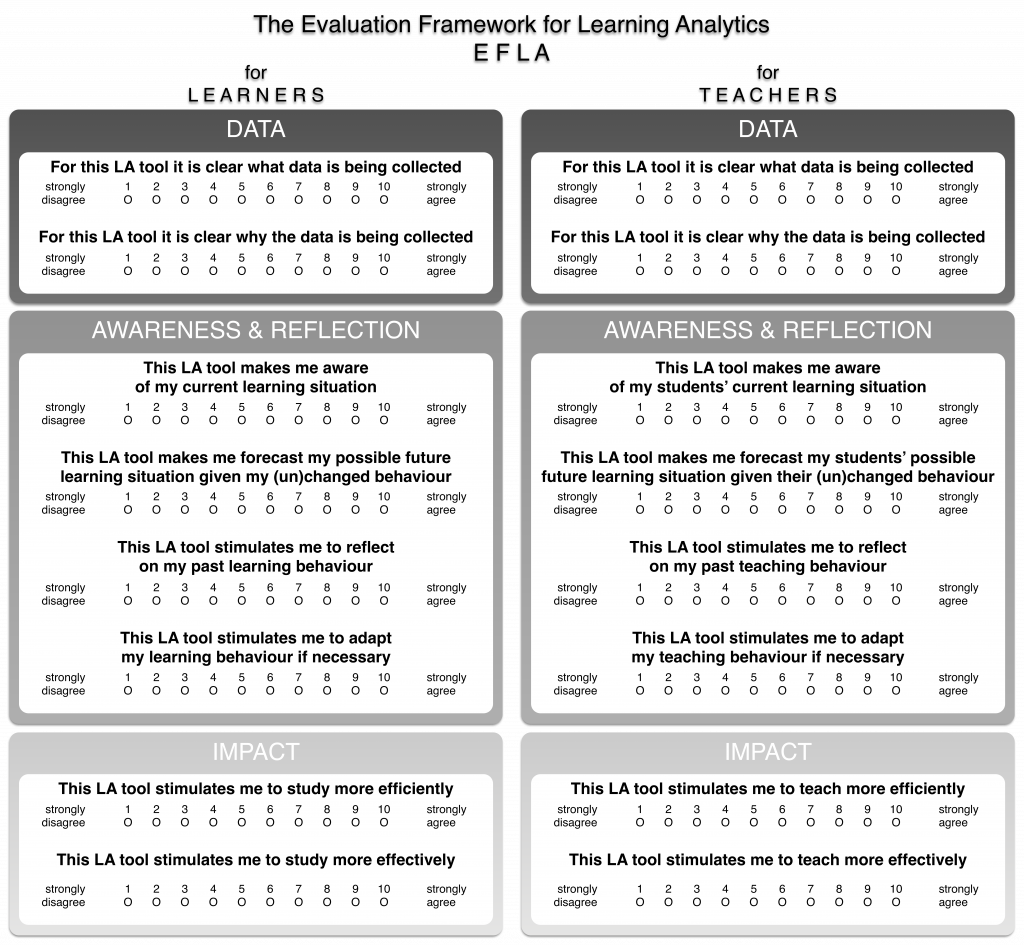
\includegraphics[width=\textwidth]{EFLA--greyscale}
        \caption{Template for the EFLA survey \cite{efla-website}}
        \label{fig:efla-template}
    \end{figure}

   The result is an online survey platform, where surveys similar to the EFLA can be created
   and hosted. While it is possible to create arbitrary survey items, some restrictions
   specific to the EFLA use-case apply (for a full list of features see table \ref{table:v1-features}).
   The original version of the survey tool is written in Python 3 and JavaScript for the server
   and user interface respectively. To be able to re-use code, the choice of language did not
   change with the new version.
   

   \begin{figure}
       \begin{tabularx}{\textwidth}{|l|X|}
            \hline
            Feature & Description \\
            \hline \hline
            Editable surveys & Edit titles, question texts and colors.\\
            Export to CSV & Export all results of a questionnaire to as CSV file\\
            Challenges & Validate data subject's email addresses. 
            White- and Blacklist email addresses. Protect surveys by password.\\
            Internationalisation & Survey items may have multiple translations.\\
            User accounts & Users may sign up and host surveys.\\
            Template surveys & Choose from a fixed set of template surveys.\\
            Visualisation & View survey results as a box plot.\\
            \hline
       \end{tabularx}
       \caption{Features of the previous version of the survey tool}
       \label{table:v1-features}
   \end{figure}

   \subsubsection{Data Model}

   \begin{figure}[H]
        \centering
        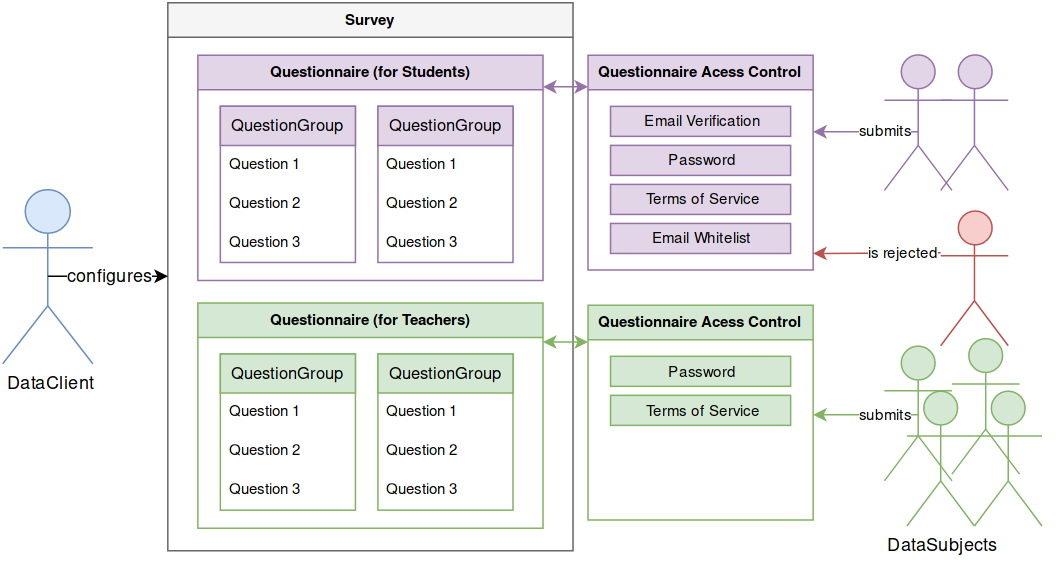
\includegraphics[width=\textwidth]{v1-model}
        \caption{Data model of the previous version}
        \label{fig:v1-data-model}
    \end{figure}

    \begin{wrapfigure}{o}{.5\textwidth}
        \centering
        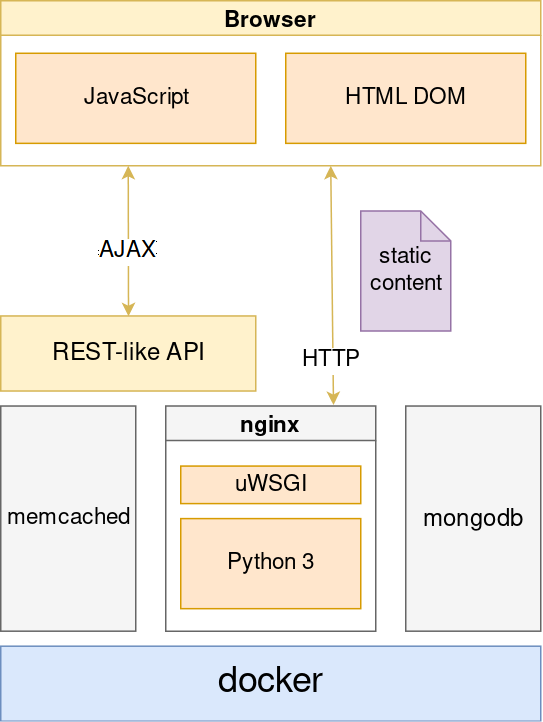
\includegraphics[width=0.4\textwidth]{v1-stack}
        \caption{Architecture overview of the previous version}
        \label{fig:v1-stack}
    \end{wrapfigure}

    The data model for the previous version is closely coupled to the specific needs of the
    EFLA survey, where a single survey consists of two questionnaires, targeting
    learners and teachers respectively.
    Each questionnaire controlls DataSubjects' rights to submit by it's own set of access 
    control modules, so that audience groups can be discriminated.
    Each questionnaire contains one or more question groups, which contains of
    one or more questions.

    \subsubsection{Architecture}
        The architecture for the previous version follows a simple client-server paradigm, where
        a web browser takes the role of the client. The server software consists of an
        application server, responding to API requests, a database and an in-memory
        key-value store for storing session data. There are two different user interfaces,
        one for data clients and one for data subjects. The data subjects' user interface
        is the page, where the survey is filled out and submitted. This page is rendered
        on the server using a templating engine and sent to the browser as a static HTML document.
        The user interface for data clients presents the user with an editor, where survey content
        can be created and modified. This user interface is realised as a one-page
        javascript application and was developed by Hannes Leutloff. Deployment is handled through
        Docker, with the help of the docker-compose tool.

\subsection{Goal}
    The goal of this thesis is to extend the functionality of the already existing
    survey tool and to contribute to the TLA ecosystem by integrating the
    survey tool as a data provider. In this thesis, the overall structure of the 
    survey platform and the server-side software stack, which was designed and developed 
    by Noah Hummel is discussed. Implementational details are discussed only 
    if they are central to the workings of the software, or solve a particular 
    conceptual challenge. The user interface was designed and mainly developed by 
    Hannes Leutloff, and is therefore not discussed here.

\subsection{Additional Contents}
\subsubsection{Source Code}
    The source code for this project is maintained at GitHub and can be found at
    \url{https://github.com/yeldiRium/st3k101}.
    The version submitted as part of this thesis is version \inline{3.1.0-beta}, 
    which can be accessed at \url{http://bit.ly/xapi-probe-3}. There, the
    source code is available as a zip-compressed archive. The reader may
    prove the authenticity of the release by calculating the archive's
    SHA-1 hash sum. \\
     
    \inline{st3k101-3.1.0-beta.tar.gz: 1f1ce2727378713bedaaf801eaa5a4d2004f9d62}
     
    \inline{st3k101-3.1.0-beta.zip: 5a38cc5e485c249c9a215b0dd997fac77cc6c595}\\[1em]

\subsubsection{Documentation}
    The source code itself is documented using docstrings and comments.
    The project's \inline{README} file is the central point of access
    for information about deployment, dependencies and development
    setup.

\subsubsection{API Reference}
    The API reference for the \inline{backend} service can be accessed
    at \url{http://bit.ly/xapi-probe-api-v6}. This version exists only
    for reference and will not be updated.
    \section{Requirements Analysis}
\label{section:requirements-analysis}

Requirements analysis was performed on the basis of previously collected use cases.
Required features and parts of the existing software that
had to be refactored were identified.

\subsection{Use Cases}

    \subsubsection{Accessing Students' Self-Regulated Learning Behavior}
    In the context of TLA, the survey tool will be used to access students' self-regulated
    learning behaviour. Several psychometrical instruments exist for this, but
    for the purpose of this thesis only instruments based on or resembling
    the motivated strategies for learning questionnaire (MSLQ) were considered.
    One such instrument described in the 1994 paper 
    ``Lernstrategien im Studium: Ergebnisse zur Faktorenstruktur und Reliabilit\"at eines neuen Fragebogens''
    (Learning Strategies in Studies: Findings on the Factor Structure and Reliability of a new Questionnaire)
     \cite{lernstrategien-wild-schiefele}
    was particularly used as a guide to define new requirements for the platform.
     
     \subsubsection{Embedding in Moodle}
     \label{use-case:embedding}
     Moodle is an LMS used at Goethe University. The platform supports embedding of external
     tools inside a course context. Because previous and simultaneous efforts by Prof. Drachsler's
     work group and collaborators already target Moodle, the new survey tool should also integrate
     with it. Surveys are still created using the survey tool's own user interface.
     Once a survey is created, it may be embedded into Moodle's course context via the LTI
     protocol. Data subjects already using the LMS may then directly participate in
     the survey without leaving the website.
 
     \subsubsection{Stand-Alone Survey Platform}
     In addition to directly embedding the survey tool into an LMS, it should be possible
     for a data subject to participate in a survey, if no LMS is used.
     This use case was carried over from the previous version.

     \subsubsection{Data Provider as Part of the TLA Ecosystem}
     As mentioned above, the survey tool will contribute to the TLA ecosystem
     by providing data to TLA's facts engine, using xAPI to communicate
     information about responses and events on the platform.

\subsection{Refactoring \& Restructuring}
\subsubsection{Database Abstraction}
The previous version of the survey tool uses a self-authored database abstraction library,
the object-document-mapper (ODM). This library is capable of persisting python objects
and relationships between them. It does this by serializing objects to JSON and storing them
using MongoDB. Runtime interactions with these objects are intercepted and converted into 
database queries using the descriptor pattern \cite{python-descriptors}.
This approach worked well for the limited use case, but it proved difficult to implement
a transaction model that follows ACID properties.
To achieve transaction safety without compromising API transparency, an existing
object-relational mapper (ORM) was chosen to replace the ODM. The key factors for the choice
of ORM were:

\begin{description}
    \item[Maturity of the project.] Data integrity is critical to the application. There is an
    increasing chance of bugs being found and resolved with increasing project age.
    \item[Support for inheritance mapping.] Not being able to effectively use class hierarchies 
    had proven itself to be a major burden on development speed during development of the previous
    version. Attributes of related classes had to be explicitely duplicated. 
    This was not only confusing to read but also difficult to maintain. 
    \item[Support for JSON or hash map columns.] JSON columns provide a convenient way to store multiple 
    translations of a text column, without producing additional joins between the main table and
    supplemental translation tables. Storing multiple representations of a string
    inside a relational database usually involves a 1-to-n relationship between
    the internationalized entity and its translations. With the use of JSON columns,
    multiple translations of a string can be stored as a dictionary inside a single
    column of the entity itself.
\end{description}

In Table \ref{table:orm-feature-comparison} a comparison between the some of the most
popular ORM libraries available for Python 3 is presented. 
Because of the project age, previous experience with the library and it's reliability 
in production environments and the large feature set, SQLAlchemy was chosen to replace the ODM.

\begin{table}
 \centering
 \begin{tabularx}{\textwidth}{|l|X|X|X|X|}
     \hline
     \diagbox{Feature}{ORM} & SQLAlchemy & PeeWee & PonyORM & SQLObject \\
     \hline
     Declarative API & Yes & Yes & Yes & Yes \\
     Eager loading of relationships & Configurable & No & Configurable & No \\
     Lazy loading of relationships & Configurable & Yes & Configurable & Yes \\
     Query caching & Yes & Yes & Yes & Yes \\
     Cascades & update, delete & update, delete & delete & delete \\
     Inheritance mapping & Yes & No & Yes & No \\
     JSON columns & Using PostgreSQL & No & Yes & Using PostgreSQL \\
     First released & 2005 & 2010 & 2014 & 2003 \\
     \hline
 \end{tabularx}
 \caption{Comparison of python ORM libraries}
 \label{table:orm-feature-comparison}
\end{table} 

\subsection{Survey Content}
 To allow other surveys apart from the EFLA survey to work well with the platform, 
 the following requirements were established:

 \begin{description}
     \item[Response ranges should be adjustable.] Responses will still be on
     a discrete scale with a step size of 1. The start and end of the scale should
     be adjustable.
     \item[Labels for the response ranges should be adjustable.] The EFLA survey
     uses the phrases ``Strongly disagree'' and ``Strongly agree'' to describe
     the lower and upper ends of the response scale respectively. As other surveys
     may use different descriptions, these descriptions should therefore be adjustable.
     \item[Question order should be configurable and optionally randomizable.]
 \end{description}

\subsection{Template Management}
The set of questionnaires which are of interest is changing over time.
Initially, the MSLQ was considered to be the main questionnaire of interest
for accessing self-regulated learning behavior. Because of the questionnaire's
size, alternatives were researched by Prof. H. Drachsler and his associates.
As new research is published and questionnaires become better statistically validated, the number of survey
 items needed to access a certain research question may decrease.
 For this reason, more current questionnaires may be preferred over
 older ones. It should be easy to integrate new survey items in the future.
 At the same time, once a questionnaire is reasonably well verified, multiple users
 may be interested in using the same questionnaire for different groups of participants.
 The previous version has rudimentary template support, but templates are supplied as static
 YAML files on build and can not be updated from the user interface.
 To overcome this limitation, the following requirements were established:

 \begin{description}
     \item[Templates should be user-contributed.] Data clients with special
     privileges, called contributors, should be able to publish new templates
     using only the user interface.
     \item[Individual survey items may be templates.] To create slightly modified
     versions of a questionnaire, it is useful to re-use existing survey items and not
     only entire questionnaires.
     \item[Templates should be modifiable after creation.] Otherwise, editing
     errors would cause the template to become unusable and the entire template
     has to be created again.
     \item[Changes should be traceable.] When the maintainer of a template 
     modifies the template, other users who own copies of it should be able to 
     review the changes.
 \end{description}

\subsection{Support for xAPI}
 The previous version only supports limited data analysis capabilities.
 The new version should interface directly with the TLA 
 infrastructure to allow for further data processing by TLA's analysis engine. 
 TLA uses the xAPI statement format as it's common data representation. To provide data
 using xAPI to TLA, the following requirements were established:

 \begin{description}
     \item[Survey results should be published to an LRS via xAPI.] A suiting xAPI 
     representation of survey results has to be defined and should be transmitted
     to the LRS vie HTTP as defined by the xAPI specification \cite{xapi-spec}.
     \item[The destination LRS should be configurable.] This allows the location
     of TLA to change in the future. It also decouples the survey tool from TLA 
     and allows interoperability with other LRSs.
     \item[xAPI statements must not be lost due to failure.] When publishing data
     to an external storage, data integrity is no longer only determined by
     database integrity. Appropriate measures must be taken to ensure 
     re-transmission in case of network failure. If transmission is not possible
     due to misconfiguration, an offline fallback method has to be provided.
 \end{description}

\subsection{Embedding \& LTI Launch}
 To achieve compatibility between Moodle and the survey tool described in \ref{use-case:embedding}, 
 the following requirements were established:

 \begin{description}
     \item[The survey tool has to implement the LTI launch protocol.] 
     The LTI launch protocol is used to embed and launch external tools 
     by the Moodle LMS. The survey tool has to recognize LTI launch requests
     and respond with an embeddable version of the survey.
     \item[Data subjects should not have to authenticate.] When using the survey tool
     from within Moodle, data subjects have already authenticated with CAS in order
     to log in to the LMS. Requiring another form of user authentication after
     this point would break the seamless user experience.
 \end{description}

 LTI uses OAuth 1 to sign requests. This provides a way for the tool provider
 to verify the identity of the LMS and the authenticity of the LTI request.
 The requirement to implement OAuth as part of this work was explicitly not required.

\subsection{Privacy Considerations}
 Since May 25th 2018, the General Data Protection Regulation has applied to EU member states \cite{gdpr-info}.
 The author is not in any way qualified to provide a legal interpretation of the regulation.
 However, in consultation with Prof. H. Drachsler, the following requirements
 were identified to conform to the regulation:

 \begin{description}
     \item[Data deletion for data subjects.] Some personal data has to be stored
     on the server in order to identify data subjects between requests. Because of the
     right to be forgotten, there has to be a way to delete personal data stored for
     a specific data subject. It is sufficient if this is not automated and can be performed
     by the site's administrator.
     \item[No user accounts are available to external data clients.] If third parties are allowed to use
     the service, it can not be guaranteed that they will follow GDPR guidelines.
     To avoid responsibility for third parties' actions on the site, there will
     be no way to sign up as a data client that does not involve contacting the administrator.
 \end{description}
 
 Other rights covered by the GDPR include the right to view and export personal data.
 Since all personal data collected is published to the TLA infrastructure,
 this will be implemented as part of the TLA infrastructure and is not
 part of the survey tool.

    \section{Concept}

\subsection{Architecture}
    The overall architecture is the same as for the previous version. The survey tool
    uses a classical client-server approach, where the client is a 
    JavaScript application running inside a web browser. This approach
    enables everyone with a modern web browser to use the platform without
    having to install any additional software locally. Notable exceptions
    are Internet Explorer, Opera Mini and the Blackberry Browser, as they
    do not fully support the CSS \inline{grid} property.
    The server-side software stack is deployed by using Docker and 
    exposed through a containerized web server.
    Communication between different containers on the server takes place
    on a virtual network which is not exposed to the internet. Communication
    between client and server is handled by a RESTful API provided
    by the server.

\subsection{Survey Content}
    During refactoring, the top-level organizational unit ``survey'' was removed
    and replaced by ``questionnaire''. Grouping multiple questionnaires
    inside a single survey only makes sense in a small set of use cases.
    For other use cases, this has proven to be confusing to users. Most of the time, 
    a survey contains only a single questionnaire. Use cases, where
    grouping of multiple questionnaires into a single survey is appropriate,
    can still be achieved by creating multiple questionnaires without any
    explicit grouping. Apart from that, the overall survey structure did not
    change significantly.

    \subsubsection{Questionnaire}
        \begin{wrapfigure}{o}{.45\textwidth}
            \centering
            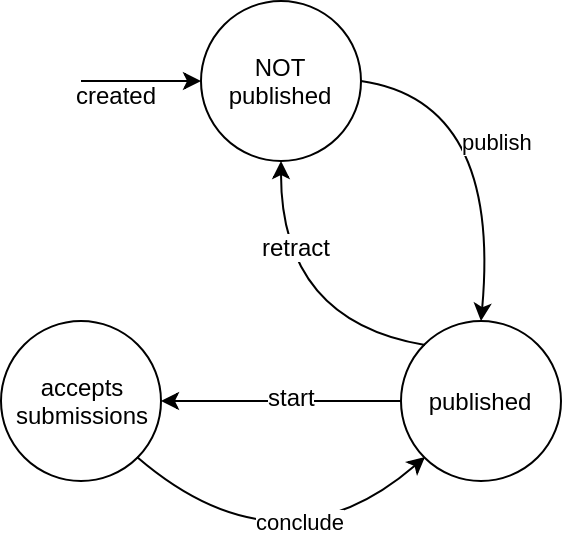
\includegraphics[width=.4\textwidth]{survey_lifecycle}
            \caption{Questionnaire life-cycle}
            \label{fig:survey-lifecycle}
        \end{wrapfigure}
        A questionnaire is a collection of dimensions, which also contains administrative
        information. A questionnaire's life cycle is modeled using three
        distinct states. The questionnaire starts out as `not published',
        which means that it is only accessible to its owner via the API
        (with the exception of templates, which will be accessible to other
        authenticated data clients)
        and will not display when accessed by data subjects via its
        public URL. This state is meant for questionnaires which are
        incomplete and being worked on. Once a questionnaire reaches its
        `published' state, it will be visible to the public via its
        public URL. It will not accept submissions via the API at this point.
        The publicly accessible representation of the questionnaire will
        not display form controls to submit and display an information
        page before accessing the survey content. This page informs the data subject,
        that submissions are not accepted at this point. Once data subjects
        are allowed to submit answers, the questionnaire enters
        the `accepts submissions' state. The public page will now display
        form controls to submit, and new submissions are accepted by the API.
        Once the survey has concluded, the questionnaire returns to
        the `published' state and can be viewed for future reference.
        If this is not wanted, the data client has the option to retract
        the survey and return it to its `not published' state.
        This life-cycle model is illustrated in Figure \ref{fig:survey-lifecycle}.

        Along with information about its life cycle, the questionnaire
        also stores information about any access control challenges
        presented to data subjects. As in the previous version, challenges
        are presented as additional form inputs when submitting. 
        In contrast to the previous version, email addresses are now always
        validated when submitting by sending a one-time-use token to the
        entered email address.
        Data clients may choose from these challenges:
        
        \begin{description}
            \item[Password:] A password has to be entered in order to submit.
            The password is chosen by the data client.
            \item[Email whitelist:] Only emails that are present in a list
            of email addresses are allowed to submit. The email whitelist
            also supports wildcard expressions to allow all email addresses
            following a certain schema.
            \item[Email blacklist:] The same as email whitelist, but instead
            of allowing certain email addresses, this blocks certain addresses
            from participating.
        \end{description}
        
    \subsubsection{Dimension}
        A dimension is a collection of questions usually pertaining to
        a specific topic. The only additional piece of information
        handled by the dimension is whether the order of its questions
        should be randomized when the survey is taken.

    \subsubsection{Question}
        A question is a single statement to which the data subject may respond
        on a numerical scale. The lower and upper bounds of this scale,
        as well as the descriptions for these bounds may be adjusted by the data client. 
        Individual questions may be used as templates,
        which is why the information on the lower and upper bounds and scale
        labels is stored on a per-question basis. Convenience workflows
        for updating this information for an entire dimension allow
        easy editing despite the large granularity of this approach.

\subsection{Internationalisation}
    Every time an API request is made,
    a request language is determined by the server and the request is
    handled in this language.
    For human-readable attributes of survey items, multiple translations
    may exist. When a survey item is created, the language it is created
    in becomes the item's original language. Translations in different
    languages may be added later by updating the survey item using 
    the desired language as the request language. 
    When no translations for the requested language exist, survey items 
    are instead served in their original language.
    To communicate information about existing translations and
    what translation was served, the API includes the item's
    current language, the original language and a list of available languages
    in the JSON representation of the item.

\subsection{Ownership, Parties, Roles}
    To control API access to survey items, these had a single
    owner in the previous version. `Owner' refers to a data client with access
    to the resource. In the next version, the ownership model
    was expanded to allow n-to-n relationships between owning parties
    and owned resources. In addition, ownership is no longer restricted to
    data clients. These changes became necessary for two reasons.
    Survey items are no longer the only resource with access restrictions,
    as will become clear in Section \ref{section:modification-tracking}.
    While survey items usually only have a single owner, i.e. the author, 
    tracking information has to be accessible to all parties sharing
    read access to the tracked resource. Because of the template management,
    data clients may have read access to survey items, of which they're not
    the author (templates). This requires a single resource to have multiple owners.
    Of course, a party may own more than a single resource, hence the n-to-n
    cardinality of this relationship. The reason for expanding ownership
    to data subjects is that this mechanism makes it easy to identify personal
    data. Data subjects own all resources which contain
    personal data. The ``right to be forgotten'' may then be implemented by
    simply retrieving all owned objects for a given data subject and deleting 
    them from the database.

    For some privileged users, access control should not be enforced.
    Also, the right to publish templates is reserved for a select
    group of users. To accomplish different levels of privilege,
    roles were introduced to all parties. A party may have a number
    of different roles, depending on the actions they're allowed to take and
    the data they'e allowed to access. There are currently five different roles:

    \begin{table}[H]
        \begin{tabularx}{\textwidth}{|l|l|X|}
            \hline
            Role & ID & Description \\
            \hline \hline
            Root & 0 & All available access control methods grant access to users with this role. \\
            Admin & 10 & An administrative user, who may view and modify other user's data in order to ensure proper operation of the platform. \\
            Contributor & 20 & A user who may make survey items available to other users as templates. \\
            User & 30 & A regular user who may create and modify their own survey items. \\
            Unprivileged & 40 & A user who may view and participate in published surveys, but not create or modify survey items. This role is used for all data subjects.\\
            \hline
        \end{tabularx}
    \end{table}

    Access control may then be enforced by checking whether the role required
    for a certain action is held by the user in question.

\subsection{Modification Tracking}
\label{section:modification-tracking}
    To track modifications of survey items, every time a modification
    is made to an item, a record of this modification is stored in the
    database. To keep storage space needed for this feature to a minimum,
    only the most recent modification for each attribute is stored.
    In the course of development, it was discovered that different kinds of modifications
    require different information to be stored in order to create a meaningful
    record of the change, which can also be presented to the data client.
    Such information includes the modified item, the modifying data client,
    previous and new values, as well as the point in time when the modification
    occurred. Five different types of records were identified:

    \begin{table}[H]
        \begin{tabularx}{\textwidth}{|l|l|X|}
            \hline
            \# & Description & Stored information \\
            \hline \hline
            1 & An attribute was updated  & Modified item, modifying data client, attribute name, previous value, new value, timestamp \\
            2 & A language map was updated & Modified item, modifying data client, attribute name, modified language name, previous value, new value, timestamp \\
            \hline
            3 & A child item was added & Parent item, modifying data client, child item, timestamp \\
            4 & A child item was removed & Parent item, modifying data client, child item name, timestamp \\
            \hline
            5 & A questionnaire was removed & Name of the questionnaire, modifying data client, timestamp\\
            \hline
        \end{tabularx}
    \end{table}

    The modified item is stored as a reference to the actual record of the item in the database.
    This makes it possible to quickly find the modified item based on
    a tracking record. In the user interface, this is used to display the
    modified item as a clickable link, which will instantly show the modified item.
    For types of modifications, where an item was deleted, this 
    kind of data model is not applicable, as the referenced record will no longer 
    exist in the database. In these instances, only the name of
    the item is stored. A special case exists for the deletion of questionnaires,
    as they do not have the parent item needed to construct the tracking record.
    In this case, only the questionnaire name is stored.
    To deliver a personalized stream of modifications to data clients,
    including only those modifications which are of interest to them,
    tracking records also use the ownership model.
    Tracking records are owned by all parties interested in the tracked
    item.

\subsection{Template Management}
\label{concept:template-management}
    A template refers to a survey item, from which other survey items
    may be created as copies. A copy of a template should always
    mirror the template's content, including its relationships
    to its children, as the children are part of the item's content.
    This is true, since all parent-child relationships 
    of survey items are aggregations; a dimension has no purpose
    without questions and a questionnaire has no purpose
    without dimensions. Every survey item may optionally also
    be a template. Survey items may be made available as a template by 
    any data client who has at least the \inline{Contributor} role.
    Templates are visible to all data clients.


\subsection{xAPI Support}
    \subsubsection{Introduction to xAPI}
        xAPI, formerly known as TinCanAPI, is a data exchange
        standard closely resembling activity streams \cite{activity-streams}.
        It was developed by the Advanced Distributed Learning (ADL) Initiative
        as a successor to SCORM \cite{scorm,xapi-history} and allows the exchange of experiential
        information in the form of statements \cite{xapi-object-model}. These statements
        use JSON as their data format and include a minimum of three
        semantic objects, ``actor'', ``verb'' and ``object''. 
        The data is transmitted using HTTP, following REST principles.

        \begin{figure}[H]
            \begin{lstlisting}[language=JSON]
{
    "actor": {...},
    "context": {
        "contextActivities": {
            "grouping": [
                {...}
            ],
            "parent": [
                {...}
            ]
        },
        "extensions": {
            "http://activitystrea.ms/schema/1.0/place": {...}
        },
        "language": "en",
        "platform": "st3k101 via localhost"
    },
    "id": "896ef7f1-8d5c-4729-b028-e9d72df47fe8",
    "object": {...},
    "result": [
        {...}
    ],
    "timestamp": "2018-09-27T14:32:15.009513",
    "verb": {...}
}

            \end{lstlisting}
            \caption{Anatomy of an xAPI statement}
            \label{fig:anatomy-xapi-statement}
        \end{figure}
    
    An xAPI statement may also include a ``timestamp'' stating the
    issue date and time of the statement, a ``context'', providing
    additional information about the event and a ``result'', detailing
    the outcome or outcomes of the event. The format is also extensible --
    additional information can be provided in the ``extensions''
    object inside the ``context''.

\subsubsection{xAPI Statement Design}
\label{section:concept:xapi-statement-design}
    There are several actions which will trigger the sending of an
    xAPI statement:

    \begin{figure}[H]
        \begin{itemize}
            \item[1)] A data client logs in into the survey platform.
            \item[2)] A data subject launches an embedded survey.
            \item[3)] A data subject answers a single question.
            \item[4)] A data subject answers a known survey item (whole questionnaire or dimension)
            \item[5)] A data client updates the xAPI activity ID of a survey item.
        \end{itemize}
        \caption{List of cases where xAPI statements are emitted.}
        \label{fig:xapi-statement-list}
    \end{figure}

    For each of these cases, an xAPI statement had to be designed.
    All of these statements share at least some of their structure.
    The \inline{context} object of all xAPI statements emitted by the survey
    tool includes the \inline{platform}, \inline{language} and 
    \inline{extensions} attributes. The \inline{language} attribute always
    contains an RFC 5646 \cite{rfc-5646}
    compliant representation of the language the action was performed
    in. The \inline{platform} attribute always starts with the
    string \inline{st3k101}, identifying the origin of the statement.
    The \inline{platform} attribute may also include the URL
    of the source LMS in the case that LTI was used. In this case,
    the URL is appended as \inline{st3k101 via SOURCE_LMS_URL}.
    The \inline{extensions} object of the \inline{context} also
    includes a geolocation for the client in RFC 7946 compliant GeoJSON
    format \cite{rfc-7946}.
    Below is a concept for what additional data should be included in 
    the statements listed in \ref{fig:xapi-statement-list}.

    \begin{table}[h]
        \begin{tabularx}{\textwidth}{|l|l|l|X|X|X|}
            \hline
            \# & Actor & Verb & Object & Result & Context \\ 
            \hline \hline
            1 & data client & logged in & login page & - & - \\ 
            2 & data subject & accessed & questionnaire & - & - \\ 
            3 & data subject & answered & question & response value & parent dimension AND questionnaire  \\ 
            4 & data subject & answered & questionnaire OR dimension & response value & parent item, if any \\ 
            5 & data client & updated & questionnaire OR dimension OR question & new activity ID & - \\ 
            \hline
        \end{tabularx}
        \caption{Concept for information included in emitted xAPI statements.}
        \label{table:xapi-data-concept}
    \end{table}

    Objects are identified by their \inline{objectType}, \inline{type} and \inline{id} in xAPI, 
    whereas verbs are only identified by their \inline{id}. For the purpose of the
    survey tool, all objects share the same \inline{objectType}, the \inline{Activity}.
    It is common practice to use a URL as an identifier or type,
    which will return a human-readable description of the item via HTTP GET. In theory,
    there is no correct identifier to use when designing xAPI statements, as the
    standard does not prescribe the use of any specific verbs or objects. In practice,
    several registries with commonly used verbs and objects exist and should
    be consulted when choosing which identifier or type to use. This avoids re-definitions
    of already existing items and increases homogeneity among statements by
    different adopters of the standard. Examples for these registries are \url{xapi.vocab.pub}
    and \url{registry.tincanapi.com}. The verbs and objects 
    used in Table \ref{table:xapi-data-concept} had to be translated into already existing
    verbs and objects. The results are detailed in Table \ref{table:xapi-identifiers-used}.
    For some of the objects, no suitable definitions existed. For those
    objects, dummy identifiers or types were used, which follow the URL format, but use 
    \inline{http://fantasy.land/} as a prefix.

    \begin{table}
        \begin{tabularx}{\textwidth}{|l|X|}
            \hline
            Verb & Identifier \\
            \hline 
            logged in & \url{https://brindlewaye.com/xAPITerms/verbs/loggedin} \\
            accessed & \url{https://w3id.org/xapi/dod-isd/verbs/accessed}\\
            answered & \url{http://adlnet.gov/expapi/verbs/answered}\\
            updated & \url{http://activitystrea.ms/schema/1.0/update}\\
            \hline \hline
            Object & Type \\
            \hline
            login page & \url{http://activitystrea.ms/schema/1.0/page}\\
            questionnaire & \url{http://id.tincanapi.com/activitytype/survey}\\
            dimension & \url{http://fantasy.land/dimension}\\
            question & \url{http://adlnet.gov/expapi/activities/question} \\
            \hline
        \end{tabularx}
        \caption{Used xAPI verb identifiers and object types}
        \label{table:xapi-identifiers-used}
    \end{table}

    In order to correlate objects in emitted xAPI statements with survey
    items in the survey tool, all survey items have a user-modifiable
    xAPI activity ID associated with them. This identifier is
    used as the object's \inline{id} in xAPI statements.
    These identifiers are not modifiable in copies of templates,
    which means that all instances of a copy will use the same xAPI
    activity ID. This is useful for conducting meta-analyses, where
    all results for a certain template could be included in the analysis,
    regardless of who conducted the survey. During testing, this
    became an issue, because the results for the same template,
    which were collected by different data clients, would not be distinguishable,
    as they all used the same identifier. For this reason,
    the email address of the data client conducting the survey
    is added as a prefix to all xAPI activity IDs before sending.
    In Figure \ref{fig:example-xapi-activity-dimension}, an example
    of how survey items are represented in xAPI is given. 

    \begin{figure}
        \begin{lstlisting}[language=JSON]
"object": {
    "definition": {
        "description": {
            "en-US": "This is a particular scale of a survey, it usually contains multiple questions."
        },
        "name": {
            "de": "5. Anstrengung"
        },
        "type": "http://fantasy.land/dimension"
    },
    "id": "<bla@blubl.net>:lernstrategien_wild_schiefele--5_anstrengung",
    "objectType": "Activity"
}
        \end{lstlisting}
        \caption{Example of how a dimension is represented as an xAPI acitivity object}
        \label{fig:example-xapi-activity-dimension}
    \end{figure}

    Actors may be represented in four different ways using xAPI. 
    The identifying feature is either the person's email address in the case
    of the \inline{mbox} and \inline{mbox-sha1sum} actor types, an account ID 
    in combination with a URL where the account is located in the case of the 
    \inline{account} actor type
    or an OpenID identity in the case of the \inline{openid} actor type.
    Data clients are represented as \inline{mbox} actor types, while data subjects may 
    be represented by as \inline{mbox-sha1sum} actor types
    or, in the embedded use-case, as an \inline{account} actor type using their
    LTI user identifier. The latter is necessary, because the email address might not be available
    through LTI. Contrary to prior expectations, the LTI user ID is not
    useful for data analysis, as Moodle will use the user entity's database ID.
    Moodle does, however, communicate a username via LTI, which for the specific Moodle instance
    at Goethe University is the same as the data subject's CAS ID.
    To retain compatibility with other LMSs while taking this finding into account,
    the username will take precedence over the LTI ID, if present in the LTI request.
    The LTI ID is also not globally unique, as there may be separate LMSs which
    use the same IDs for different users. For this reason, the LTI user ID is
    prefixed with the identifier of the source LMS, which is always present in LTI requests.

    The recipient of the statements is determined by the object which is acted upon. 
    This makes intuitive sense, as the person owning a specific survey item is the one interested in
    collecting data on it. At the highest level, all survey items are
    organized into one questionnaire and there is no use-case for different
    data consumers for individual parts of the questionnaire. 
    For this reason, recipients are configured on a per-questionnaire basis.
    For objects which do not have an owner, e.g. the survey tool's login
    page, a default recipient is configured system-wide.
    To recover from failure in the case that an xAPI statement
    can not be transmitted over a prolonged period of time, the
    statement as well as the recipient and timestamp of the failure
    are logged to file and may then periodically be recovered.

\subsection{Support for LTI}
\label{section:concept:lti}
    The embedded user interface is launched by the LMS using the LTI protocol.
    To identify the source LMS, a random token, the consumer key,
    is generated in the back-end for every questionnaire. To
    embed a questionnaire within the course context, an LTI request
    with the correct combination of request URL and consumer
    key has to be made by the LMS.
    Information about the user is already present in the
    request body and is used to identify the data subject. 
    Since there's some time between the LTI launch request
    and survey submission, user information
    has to be stored on the server for this period of time.
    To achieve this, the required data is stored in the data subject's account.
    If a data subject accesses the service through LTI for the first time, 
    a new account is provisioned for them.
    When launching the survey tool via LTI, a session is created
    for the data subject and a session token embedded into
    the user interface. Actions by the data client in the
    embedded user interface will use the embedded session token
    for authentication with the API. This mechanism allows
    the API to identify the data subject on every subsequent
    request. A valid LTI request is treated as sufficient
    authentication for the data subject, as the source LMS already
    authenticated the user prior to them accessing the questionnaire.

\subsection{Email validation}
    When data subjects participate in a standalone survey,
    it is difficult to recognize repeated submission by the same
    person. Most features used for identification, e.g. the client's
    IP address or cookies present in the browser, can easily be
    modified by the data subject. Even more
    advanced measures, such as browser fingerprinting, are ultimately
    controlled by the client, as communication with the server
    is handled by a publicly available API. For this reason,
    a third party has to be involved in validating the user's identity.
    The survey tool achieves this validation through email.
    When submitting responses, the data subject has to enter their
    email address. At this point, the responses are stored on the server,
    but no xAPI statements have been emitted and the responses do not
    yet count towards the generated statistics. 
    A randomly generated token is embedded into a URL pointing back to the survey tool. 
    This URL is then sent to the submitted email address. 
    Once the data subject follows the URL, the server will associate the 
    token with the user's responses in order to validate them.
    After validation, the appropriate xAPI statements are emitted.

\subsection{Privacy Considerations}
    As mentioned in Section \ref{section:concept:lti}, when a data subject participates
    in a survey, a user account is provisioned for them. Removal
    of this account and all associated personal data may be performed
    via the API when authenticated as an admin user.
    In order for the admin to know which account to communicate
    to the API, the API allows admin users to query for existing
    user accounts. Data removal is limited to admin users,
    as removal of accounts by data subjects themselves would require
    some sort of authentication mechanism for data subjects.
    When an email address is present for the data subject,
    authorization via email is a possible solution for this.
    In this scenario, the data subject would receive an email
    with a randomly generated token, which can be used to remove their personal
    data. If there is no email present for the data subject, say,
    when the account was provisioned using LTI, or if the data subject
    does not have access to their email account, this mechanism fails.
    For this reason, email as the sole mechanism for data removal is not a viable
    option at the moment.
    
    \section{Implementation}
\label{section:implementation:architecture}
\subsection{Architecture}
    \begin{figure}[H]
        \centering
        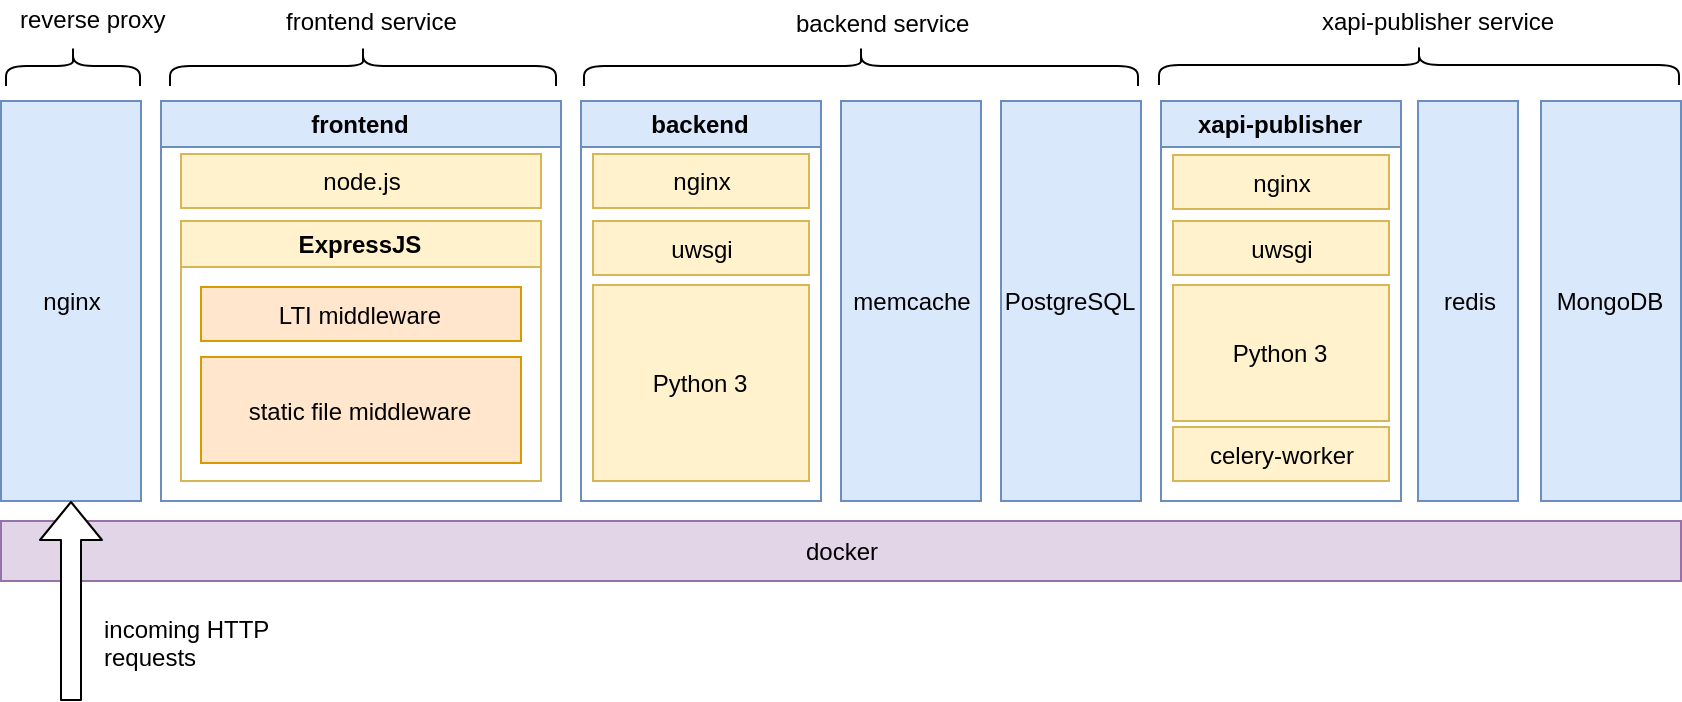
\includegraphics[width=\textwidth]{stack}
        \caption{Server-side software stack}
        \label{fig:stack}
    \end{figure}

    The server-side architecture is composed of multiple services.
    The ``frontend'' service is responsible for serving the
    user interface statically and intercepting LTI requests.
    The ``backend'' service is responsible for serving the API,
    user and session management and communication with the database.
    The ``xapi-publisher'' service is responsible for transmission
    of xAPI statements generated by the backend service.
    Each service uses slightly different technologies, depending
    on the requirements of the service. The API and ``frontend'' service
    are exposed through an nginx web server, which acts as a reverse
    proxy, forwarding incoming HTTP traffic to the appropriate docker
    containers.

    \subsubsection{The Backend Service}
        The backend service is implemented using the Flask
        library, which allows Python to interface with a web server
        using the web server gateway interface \cite{pep-333}. Similar
        to PHP or CGI extensions, the nginx web server will accept incoming
        requests. It will then, using uWSGI, fork a python interpreter
        which will respond to the request. This means that no data
        can be persisted in the Python application itself, as the
        Python context will be discarded for every request.
        To persist data, a PostgreSQL database and a memcached
        in-memory key-value store are used.
        Persistent data, such as survey content, is stored
        in the database, whereas semi-persistent data, such as user
        sessions, is stored in memcached. This design allows
        for horizontal scalability, as multiple instances of the
        \inline{backend} container can be used with the same database.
        No data dependencies exist between the \inline{backend} containers.
        The only bottleneck in this scenario is the shared database.
        This could be solved in the long-term by replacing the single PostgreSQL
        instance by a database cluster.

    \subsubsection{The Frontend service}
        The frontend service consists of a simple node.js
        application running the ExpressJS web server. For the
        web server, two middlewares are provided, one for
        serving static files and another for intercepting LTI launches.
        This is necessary as the user interface has to be
        parameterized for each LTI launch before serving it to the data client.

    \subsubsection{The xAPI-Publisher Service}
        The xapi-publisher service closely mimics the design of the
        backend service. In addition to Flask and uWSGI,
        it also runs several worker threads, which are responsible for the
        asynchronous sending of xAPI statements. Since xAPI statements
        are JSON documents, a document based database - MongoDB - is used instead
        of a relational database to persist xAPI statements between requests.
        For inter-process communication between web server and
        worker threads, a task queue consisting of the Celery library
        and the redis in-memory database is used.

        \begin{wrapfigure}{o}{.5\textwidth}
            \centering
            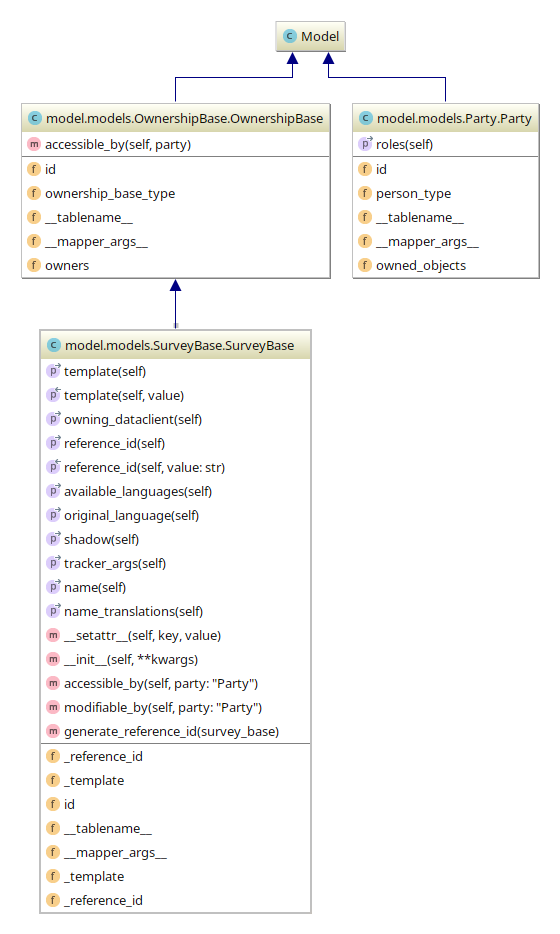
\includegraphics[width=0.49\textwidth]{base-classes}
            \caption{The three main base classes}
            \label{fig:base-classes-dia}
        \end{wrapfigure}

        The functionality provided by the xapi-provider service
        is separate from the backend service, duplicating
        most of the architecture already present. This might at first seem
        less than optimal, as it violates the DRY (don't repeat yourself)
        principle to the extent that configuration for two separate containers
        has to be created and maintained. It does, however, allow for better
        separation of concerns. The backend container already
        handles business logic and user management. A unique
        set of challenges exists that has to be solved for publishing xAPI
        statements, which would unnecessarily increase the complexity
        of the backend service. One such challenge is that
        data needed to create an xAPI statement is sometimes present in a request
        before the data is actually valid and should be transmitted. 
        When a data subject answers a survey using the stand-alone survey
        interface, their answers are submitted to the server but only
        become valid once they have verified their email address.
        The required data to build the xAPI statement, including the data
        subject's IP address, has to be stored on the server until this
        point. In order to avoid convoluting the backend service's
        data model and business logic to account for this, a separate
        service solely responsible for temporarily storing and safely 
        transmitting the xAPI statement is used.
        This allows the backend service to only use minimal logic
        for communicating with the xapi-publisher service.
        It also allows maintainers of the codebase to make changes
        to the publishing behaviour without having to know the internal
        workings of the backend service.

\subsection{Data Model of the \inline{backend} service}
    \subsubsection{Class Hierarchy}
        The class hierarchy is centered around three abstract base classes,
        \inline{SurveyBase}, \inline{OwnershipBase} and \inline{Party}.
        \inline{OwnershipBase} is the base class used for all classes
        which can be owned by a \inline{Party}. \inline{Party} is
        the base class used for all user-type classes. \inline{SurveyBase}
        is the base class for used for all survey items.
        Each of these classes provides common functionality and
        interfaces to their subclasses.

        \begin{figure}
            \centering
            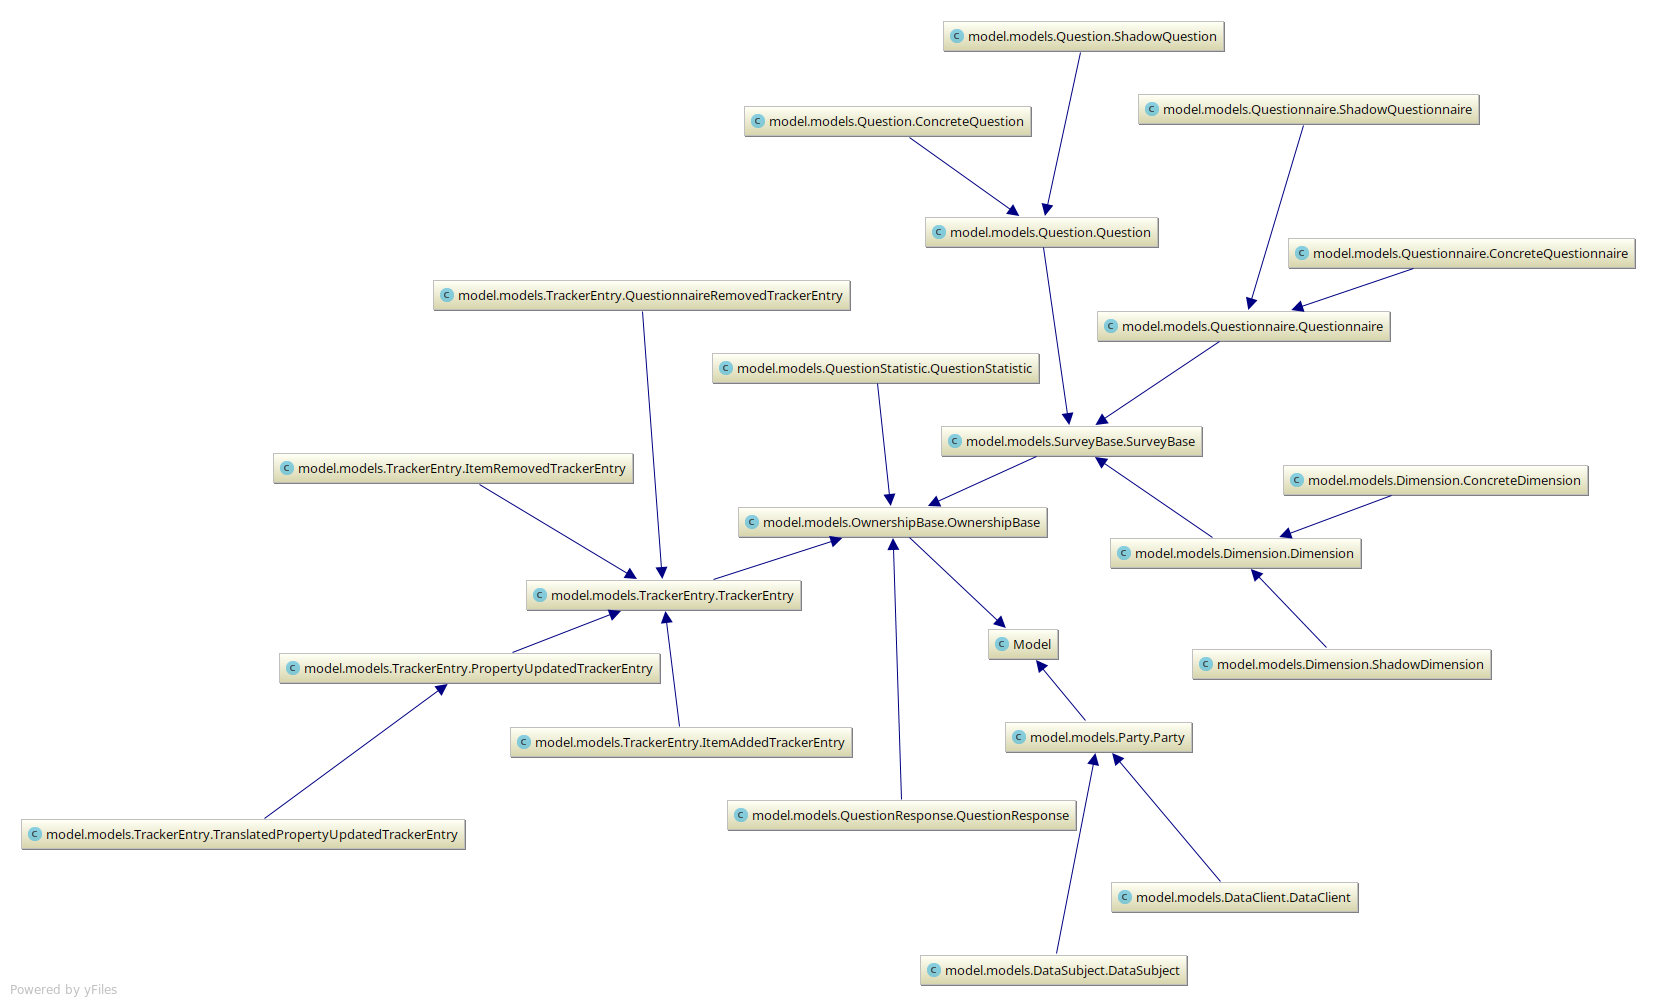
\includegraphics[width=\textwidth]{models}
            \caption{Model class hierarchy}
            \label{fig:model-dia}
        \end{figure}

    \subsubsection{Inheritance Mapping via SQLAlchemy}
    \label{section:implementation:inheritance-mapping}
        The SQLAlchemy library provides three distrinct mechanisms
        for mapping class hierarchies to relational database schemas,
        \textit{joined table inheritance}, \textit{single table inheritance}
        and \textit{concrete table inheritance}.
        Joined table inheritance uses a separate table for every
        class along the hierarchy, with each table only
        containing data declared by the corresponding class.
        Attributes inherited from superclasses are associated
        with subclasses by one-to-one relationships between the
        superclass table and subclass table. When loading
        an instance of a subclass, a join statement is generated,
        which also loads the appropriate record from the superclass
        table. Single table inheritance uses a single table
        for all subclasses of a certain class. Fields
        not used by a certain subclass are populated with \inline{NULL}
        values. Concrete table inheritance uses a separate table for
        every class, which contains all the data needed to load an
        instance of the class. This means that inherited attributes
        will be duplicated in subclass tables.
        From a performance perspective, single or concrete table
        inheritance outperforms joined table inheritance, since
        no join operation is needed to load an instance.
        From a storage perspective, joined table inheritance is
        optimal. Since SQLAlchemy does not support as many
        operations on concrete table inheritance as for the
        other types of inheritance mapping \cite{sqla-inheritance}, concrete inheritance
        mapping was not used. While single table inheritance
        works well for shallow class hierarchies, more
        complex hierarchies with multiple levels of inheritance
        produce only sparsely populated database records, as more attributes
        will be unique than shared for most classes.
        For the survey tool, this approach would only create
        two tables. For storage optimization, the joined
        inheritance approach was used.

    \subsubsection{Template Management - The Template Triad}
    \label{section:implementation:template-triad}
        \begin{figure}
            \centering
            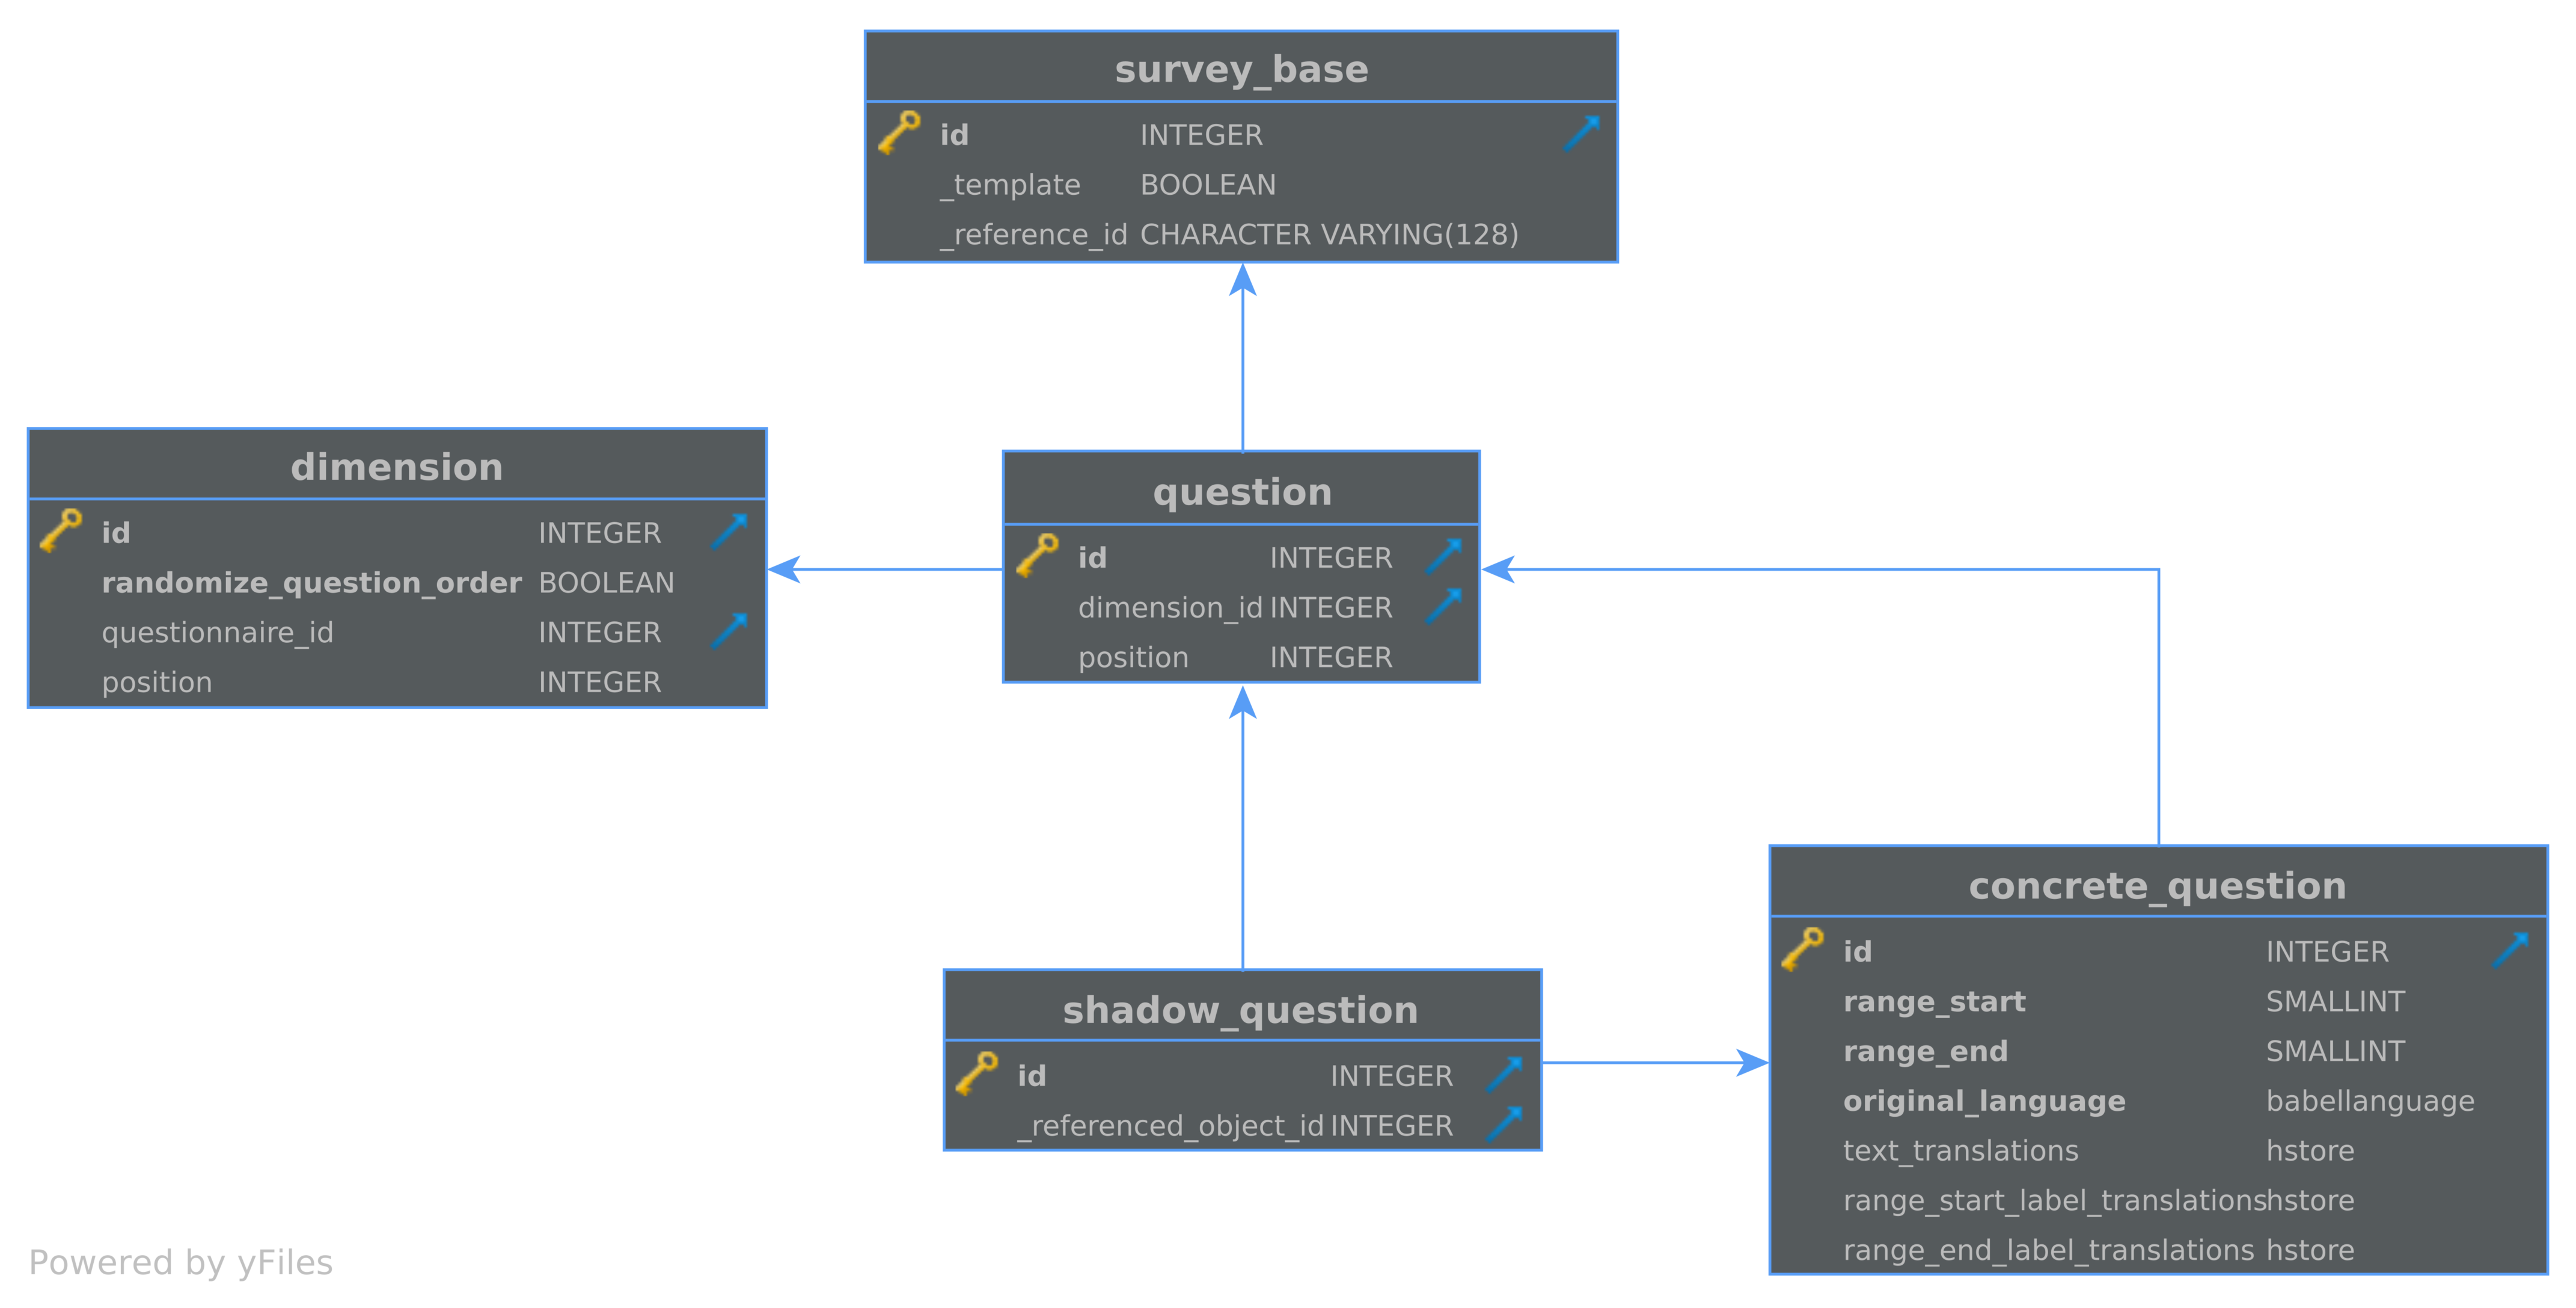
\includegraphics[width=\textwidth]{schema-shadows}
            \caption{Database schema for a single question including foreign key constraints}
            \label{fig:schema-shadows}
        \end{figure}
        \begin{figure}
            \centering
            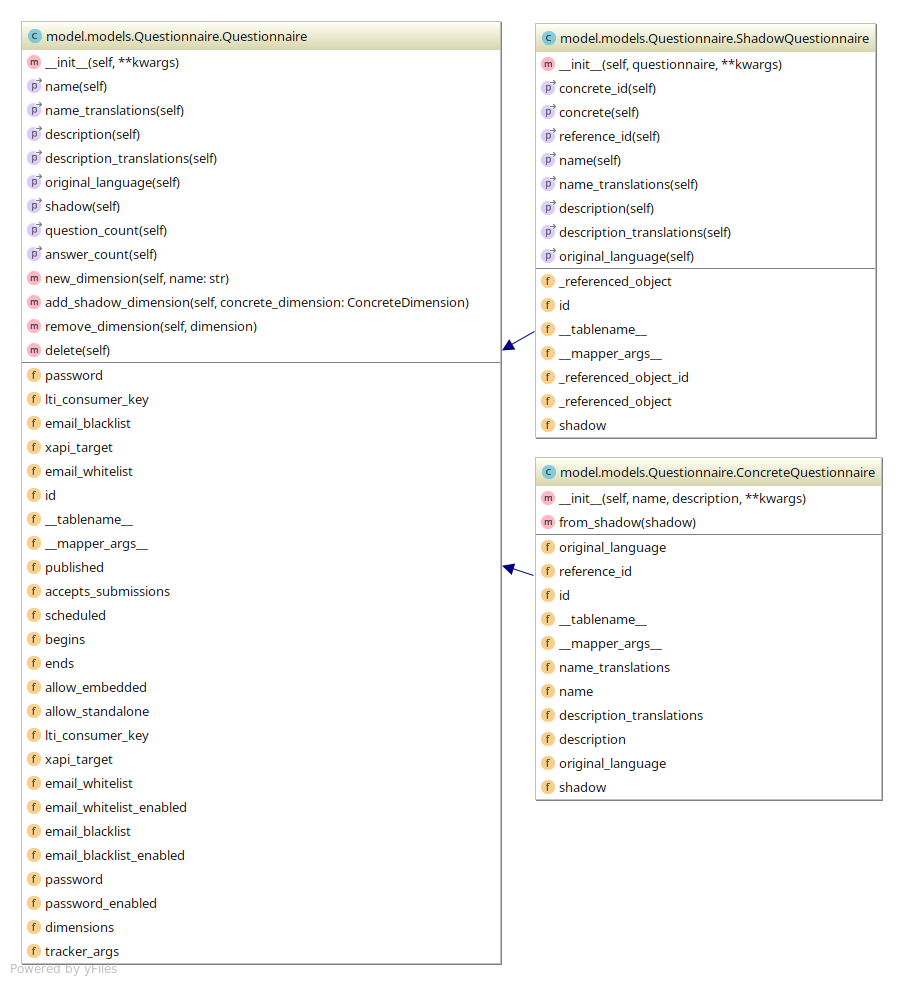
\includegraphics[width=.9\textwidth]{questionnaire-dia}
            \caption{The template triad, exemplarily depicted by the questionnaire data model}
            \label{fig:questionnaire-dia}
        \end{figure}

        To allow user-contributed templates which may also be modified after
        creation, the same data structures are used for templates as for
        regular survey content. Creating copies of these templates is done by
        reference instead of physically copying the template's content.
        This is because template content may be modified
        at any time, and these modifications have to be propagated to
        all existing copies. If copies were created by physically
        copying the template's content, updating a template would
        also cause all copies to be updated in the database. The
        asymptotic number of block accesses of this approach scales linearly
        with the number of copies present and potentially produces
        join operations with large result sets. It also stores
        large amounts of redundant data.Copies, though, are
        proxy objects, which delegate read operation to the referenced
        template. Survey items containing actual data are called
        concrete instances, whereas copies which do not contain
        the actual data are known as shadow instances.
        For each direct \inline{SurveyBase} subclass, \inline{Questionnaire}, \inline{Dimension}
        and \inline{Question}, there are two more subclasses for the concrete and shadow
        representations of the class. this \textit{template triad} is depicted in 
        Figure \ref{fig:questionnaire-dia} and \ref{fig:schema-shadows}. For the sake of brevity,
        the direct descendents of \inline{SurveyBase} will be called the \textit{super-classes},
        while its descendents will be addressed by \textit{concrete} and \textit{shadow}
        respectively. For template management,
        each of these classes fulfils a specific role. All actual data is stored
        in the concrete- and super-classes, while shadow-classes only
        contain a reference to a concrete. As shown in Figure \ref{fig:questionnaire-dia},
        some data is stored in the super-class instead of the concrete class.
        The reason behind this design is, that some attributes of shadow classes
        may still be modified and should not just reflect the state of the associated
        concrete. An example of this is the access control configuration
        of the \inline{Questionnaire} class. Data stored in the concrete
        class can be categorized as \textit{survey content}, while data
        stored in the super-class can be categorized as \textit{administrative data}.
        The super-class also acts as an interface for the concrete and shadow classes,
        specifying all accessors that should be available for its subclasses.
        The shadow classes act as proxies, which use Pythons \inline{@property}
        decorator to provide transparent read access to the referenced concrete's
        attributes.

        \begin{wrapfigure}{o}{.5\textwidth}
            \centering
            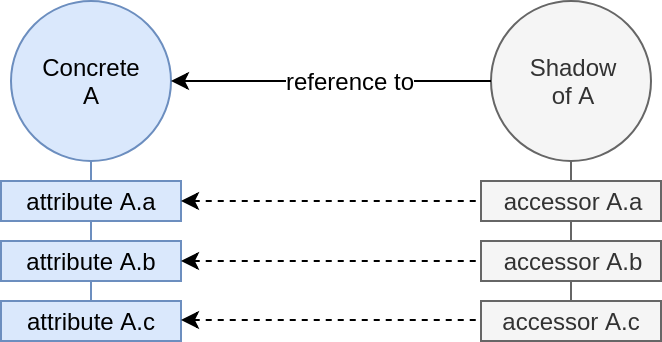
\includegraphics[width=.48\textwidth]{shadow-concept}
            \caption{Schematic depiction of the relationship between concrete \& shadow instances}
            \label{fig:shadow-concept}
        \end{wrapfigure}

        \begin{figure}[H]
            \begin{lstlisting}[language=Python,frame=lines,backgroundcolor=\color{background},firstnumber=285]
@property
def reference_id(self) -> str:
return self._referenced_object.reference_id

@property
def name(self) -> str:
return self._referenced_object.name
            \end{lstlisting}
            \caption{Example of transparent proxying of concrete attributes in shadow classes}
        \end{figure}

\subsection{Template Management}

    \subsubsection{Creation of Shadow Instances}
        Creating a shadow instance from a concrete instance not having
        any relationships to other items is trivial.
        When creating a shadow instance from a concrete instance
        which has children, the resulting shadow
        instance should also duplicate the relationship structure
        of the reference concrete instance. In Figure \ref{fig:concrete-shadow},
        an example for this is given. In the example, Shadow A
        was created from Concrete A. Parent-child relationships
        are modeled as a directed graph with edges from parent to child for the 
        purpose of this example. The creation of Shadow A will cause the
        entire subtree starting from concrete A to be duplicated
        with shadow instances, pointing to their corresponding
        concrete counterparts. The result is a copy of the
        concrete instance and its relationship, which is always
        in synchronism with its source, but can not be modified.

        \begin{wrapfigure}{o}{.6\textwidth}
            \centering
            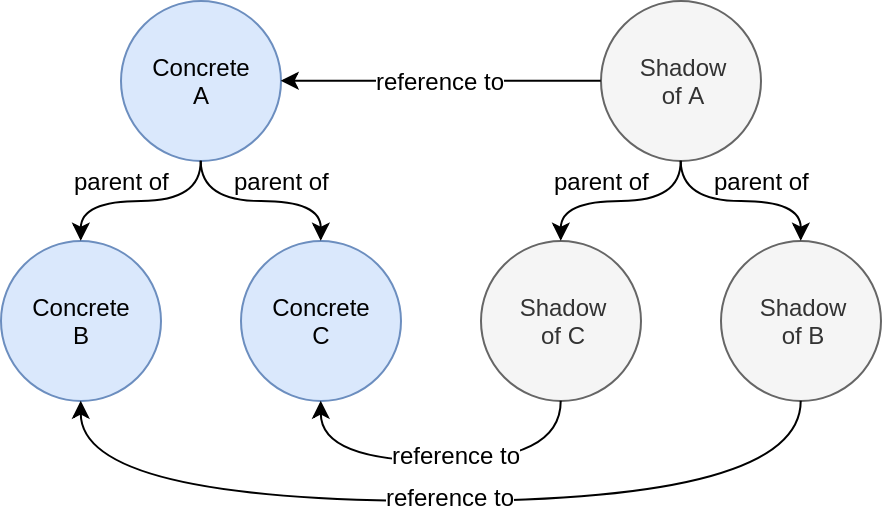
\includegraphics[width=.58\textwidth]{concrete-shadow}
            \caption{Shadow instances duplicate the structure of the concrete items}
            \label{fig:concrete-shadow}
        \end{wrapfigure}

        A special case occurs, when a shadow is created from
        a concrete, whose subtree also contains shadows.
        While it would be possible for a shadow instance to reference another
        shadow instance, a shadow instance should always reference a concrete
        instance directly. The reason for this is the asymptotic number
        of block accesses needed to read from shadow instance. If a shadow references
        another shadow, the \inline{reference_to} relationship would
        have to be traversed multiple times until the concrete instance
        is found. Access times would then scale linearly with
        the degree of separation between the accessed shadow instance
        and the referenced concrete. To avoid this, if a shadow
        instance is encountered while traversing a concrete's
        subtree on shadow creation, the shadow's \inline{reference_to}
        relationship is traversed, until a concrete instance is found.
        The new shadow instance is then created as a reference to this
        concrete instance. The example in Figure \ref{fig:template-contains-copies}
        depicts this case. In the example, Shadow A was created from
        Concrete A. Concrete A's subtree contains a Shadow instance,
        Shadow \#1 of B, which should be duplicated in Shadow A's subtree.
        Instead of pointing Shadow A's right child to concrete A's left child,
        Shadow \#1 of B's \inline{reference_to} relationship is followed.
        Concrete B is encountered
        and becomes the referenced template for shadow \#2 of B.
        This approach maintains the degree of separation between shadows
        and concretes always at one.

        \begin{figure}[H]
            \centering
            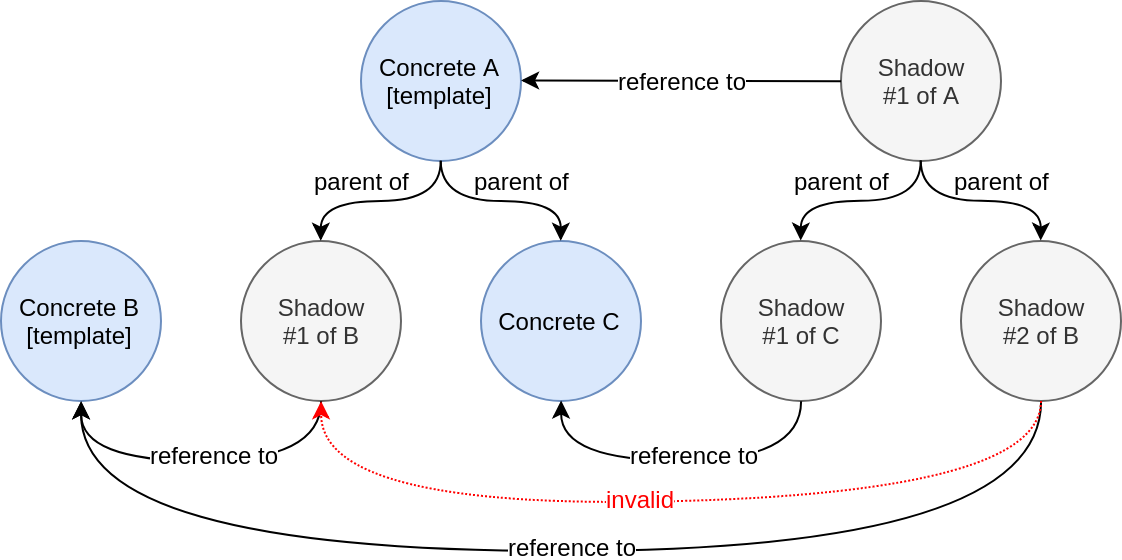
\includegraphics[width=.9\textwidth]{template-contains-copies}
            \caption{Duplication of a concrete structure which contains shadow instances}
            \label{fig:template-contains-copies}
        \end{figure}

    \subsubsection{Modification of Templates}
        Modifications of template content is trivial, as shadow instances
        will always read from the referenced template.
        When modifying a template's relationships to it's children,
        the changes have to be duplicated in all copies of the template.
        To achieve this, the \inline{reference_to} relationship is
        traversed backwards to find all copies of the template. The
        copies are then notified of the modification and apply
        it to their children as well. This operation is
        depicted in Figure \ref{fig:modify-concrete-structure}.

    \subsubsection{Deletion of Templates}
        When a template is deleted, copies of it become invalid,
        as they no longer have any instance to point to.
        Two possible solutions for this are either deleting
        all associated shadows, or converting all associated
        shadows into concrete instances. 
        The former is less complex from an implementation perspective, while the 
        latter is more user-friendly, as it does not result in unexpected 
        deletion of content. There are also use cases, where
        deleting all associated shadows might be intended,
        say, if the survey item is retracted
        and should no longer be used. There is no
        default behavior to satisfy all use cases.
        For this reason, a compromise between the two
        approaches was made. By default, when a template
        is deleted all associated shadows are also deleted.
        Contributors are therefore encouraged to edit existing
        templates instead of deleting them. Templates
        will also show a counter showing the number of
        associated shadows in the user interface, making the
        contributor aware of possible repercussions.
        If the contributor chooses to delete a template anyway,
        the modification tracking feature will provide
        accountability and transparency to the affected data clients.
        When deleting a template questionnaire, however, the
        associated shadows are converted into concrete instances,
        as the questionnaire might already be published and
        available for participation. In this case, deleting
        the questionnaire would interfere with another data
        client's survey and delete already collected results,
        which is not acceptable.

                \begin{wrapfigure}{o}{.7\textwidth}
            \centering
            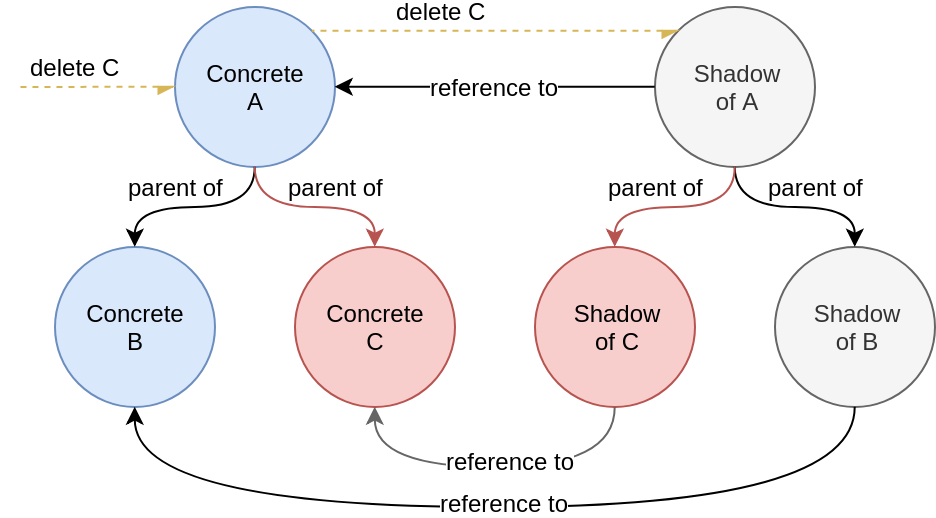
\includegraphics[width=.68\textwidth]{modify-template-structure-delete}
            \caption{Modifications of templates are relayed to copies. Items marked in red are deleted.}
            \label{fig:modify-concrete-structure}
        \end{wrapfigure}

        \begin{figure}[H]
            \centering
            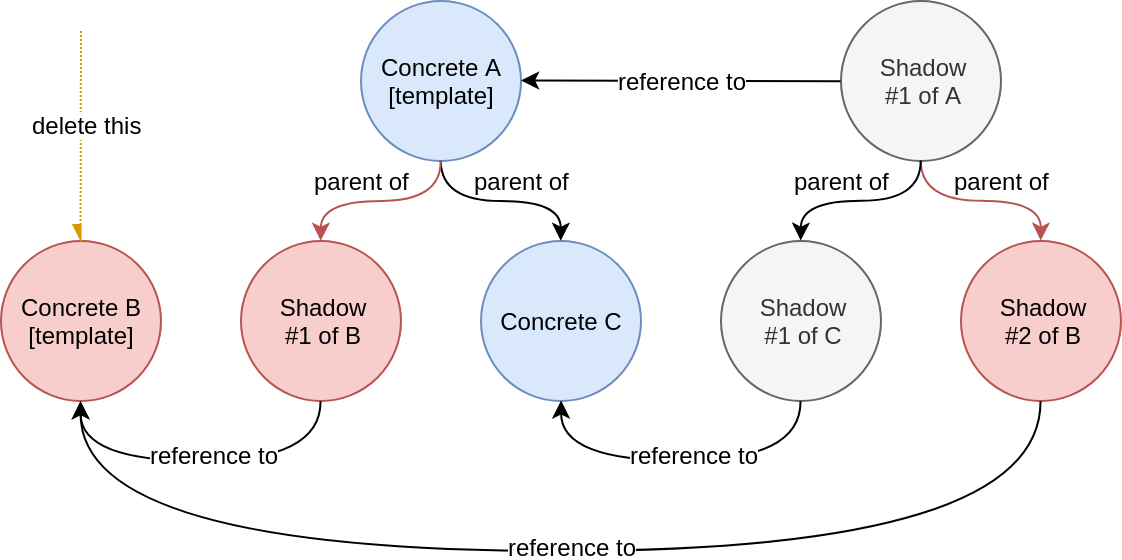
\includegraphics[width=.9\textwidth]{delete-template}
            \caption{Deletion of a template is propagated to all associated shadow instances. Items marked in red are deleted.}
            \label{fig:delete-template}
        \end{figure}

    \subsubsection{Modification Tracking for Templates}
        The modification tracker for a given data client should not 
        merely show changes to concrete instances which are owned by
        the data client. Rather, it should also include changes
        made to templates, of which the data client owns copies of.
        This provides accountability and transparency to data clients
        who choose to use templates. As changes are immediately applied
        to copies, this is an important feature for consistent user
        experience. To achieve this, every time a modification
        is made to a template, ownership of the resulting tracking record 
        is given not only to the template owner, but to all
        owners of associated shadow instances.

\subsection{API}
    The API is organized using the \inline{Flask-RESTful}
    library \cite{flask-restful}. For each type of survey item, a canonical endpoint and a set of
    contextual endpoints exist, all of which are mapped to the same handler.
    Canonical endpoints follow the \inline{http://HOST:PORT/api/TYPE/ID} format,
    where \inline{TYPE} is the type of survey item. Each survey item is identified
    by it's unique ID, which may be used for accessing the item via its endpoints.
    If a survey item has child elements, then these may be accessed by
    appending \inline{/CHILD_TYPE/} or \inline{/CHILD_TYPE/CHILD_ID} to any
    of the parent's endpoints. The former returns a list of all children,
    while the latter accesses a single child. These endpoints are called
    contextual endpoints.

    Each survey item is also associated with at least one JSON schema,
    which is used for serialization and deserialization of the classes
    instances. The schemas are implemented using the Marshmallow
    library. Each survey item's schema also includes a URL pointing to
    the canonical endpoint of the item, which may be used for
    fetching the item again in the future.

    Before any other request handler is invoked in the backend,
    information about the request language and user session are parsed.
    The request locale is determined by three mechanisms, which take
    precedence over each other in the order mentioned here
    (the latter overrides the former). First, the HTTP headers
    are inspected for the \inline{Accept-Languages} field and the best
    match is chosen from the list of available languages.
    If cookies were sent with the request, they are searched for
    a \inline{locale} cookie. Lastly, the request parameters
    are inspected for the \inline{locale} parameter.
    Session information is communicated using the \inline{Authentication}
    field of the request headers, following the bearer authentication scheme.
    If a session token is found in the HTTP headers, the token is validated.
    If successful, the associated \inline{Party} object is loaded and
    injected into the request context.    

    \subsubsection{Access Control}
        Access to API endpoints and actions is handled by two separate mechanisms.
        The first mechanism uses Python function decorators to
        block or grant access to an entire endpoint by checking the
        current user's role. The second method involves checking the
        ownership status of the accessed resource.
        Different convenience methods exist for both mechanisms. These methods are listed in Table 
        \ref{table:acl-convenience}

        \begin{table}
            \begin{tabularx}{\textwidth}{|l|l|X|}
                \hline
                Method & Arguments & Description \\
                \hline \hline
                \inline{@needs_role} & \inline{[Either Role [Role]]} & 
                Grants access to the wrapped endpoint, if the user holds all roles in the given 
                list. List items may be tuples of roles. In this case, only one of the 
                roles contained in the tuple is sufficient. The expression 
                \inline{[User, (Contributor, Admin)]} would match any user, who
                has the \inline{User} role as well as either the \inline{Contributor} or
                the \inline{Admin} role.\\
                \inline{@needs_minimum_role} & \inline{Role} &
                Grants access to the wrapped endpoint, if the role's ID value is
                less than or equal to the ID of the given role. Roles
                can be sorted by their ID, with \inline{Root} having the smallest and
                \inline{Unprivileged} the largest ID. This method is useful for
                restricting access to an endpoint to all users with a
                certain level of privilege while also allowing all users
                with a higher level of privilege. \\
                \hline
                \inline{SurveyBase.accessible_by()} & \inline{Party -> bool} & 
                Checks whether a \inline{SurveyBase} may be read by the given party.
                This methods defaults to \inline{True} for \inline{Admin} and above.
                Read access is also granted, if the \inline{SurveyBase} is a template.
                Otherwise, this method only returns \inline{True}, if the \inline{Party}
                owns the \inline{SurveyBase}.\\
                \inline{SurveyBase.modifiable_by()} & \inline{Party -> bool} & 
                Checks whether a \inline{SurveyBase} may be modified by the given party.
                This methods defaults to \inline{True} for \inline{Admin} and above.
                Otherwise, this method only returns \inline{True}, if the \inline{Party}
                owns the \inline{SurveyBase}.\\
                \hline
            \end{tabularx}
            \caption{Convenience methods for enforcing access control restrictions}
            \label{table:acl-convenience}
        \end{table}

\subsection{Authentication}
    \subsubsection{Data Client Authentication}
        Authentication for data clients can be performed by providing
        a valid combination of email and password. These parameters
        are sent to the backend in JSON format. The request
        can be encrypted by the client using TLS when a valid
        certificate is provided for the load balancer. The load balancer
        will then decrypt the request and pass it unencrypted to the backend
        on the virtual network. When creating a new data client,
        a random salt is generated using the operating system's
        random device. The provided password and salt are then hashed
        using the native Python implementation of the Argon2 password hashing function \cite{argon2}.
        The password hash and salt are stored in
        the database and can be used to validate login attempts
        by re-applying the hashing algorithm to the salt and the provided
        password, and comparing the resulting hash with the stored hash.

    \subsubsection{Session Management}
        Once a \inline{Party} has been successfully authenticated, a \textit{session record}
        is created and published to the \inline{memcached} instance.
        This session record includes information about the
        \inline{Party}, a timestamp of the last performed action by the \inline{Party}
        and a randomly generated \textit{session token}.
        The session token is handed out to the client via the API
        and may be used by the client to identify itself
        in subsequent requests. Every time the session token is used
        in a request, the timestamp stored in the session record is
        updated to the current time. If the difference between
        the timestamp and the current time exceeds a certain limit
        in any request, the token is rejected and the session record
        is removed from \inline{memcached}. This ensures the eventual
        removal of unused session records from the cache and protects
        the user against re-use of their session token if they forgot
        to log out. Another protection against token stealing
        is IP pinning. When a user is successfully authenticated,
        their IP address is included in the session record.
        If any subsequent request with the associated token
        uses a different IP address than was used for authenticating,
        the token will be rejected and the session will be removed
        from the cache.

\subsection{Support for xAPI}

        \begin{wrapfigure}{o}{.5\textwidth}
            \centering
            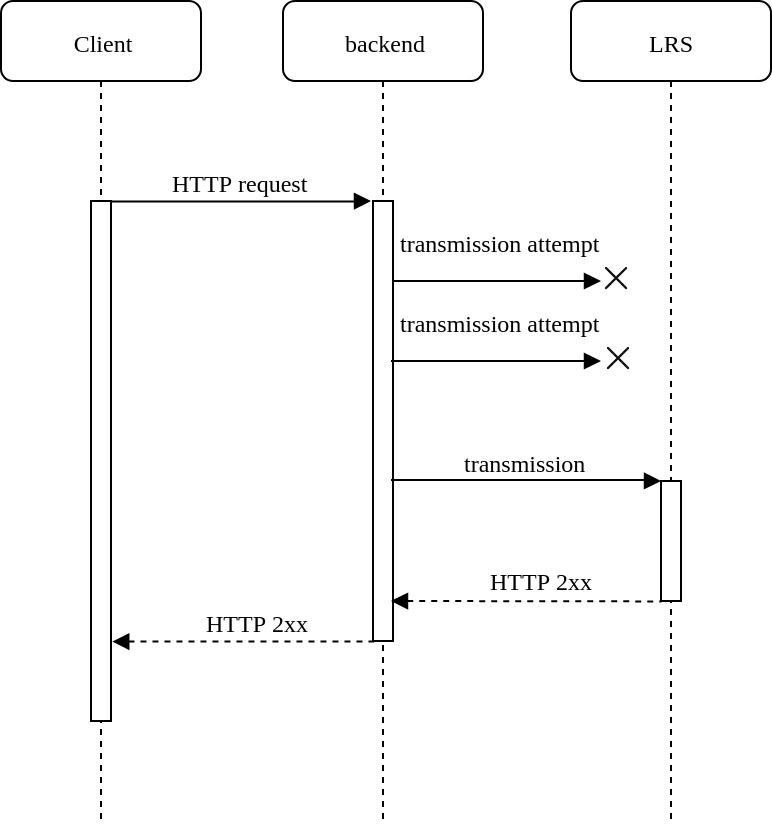
\includegraphics[width=.48\textwidth]{synchronous-xapi}
            \caption{Synchronous (blocking) transmission of xAPI statements}
            \label{fig:synchronous-xapi}
        \end{wrapfigure}
        
    \subsubsection{xAPI in the Backend Service}
        xAPI statements are created in the backend service using an
        object-oriented API. Statements are queued locally using
        the \inline{XApiPublisher} class, which acts as a transaction manager
        for xAPI statements. When a request context is created by the
        WSGI middleware, a new transcation is started. 
        Queued statements are only sent to the \inline{xapi-publisher} service, 
        when the transaction is committed at any point during handling 
        of the request. By default, when the request was handled
        without raising an error, and a rollback was not explicitly
        executed during the request, the transaction is committed automatically
        at the end of the request.

    \subsubsection{The xAPI-Publisher Service}

        \begin{figure}
            \centering
            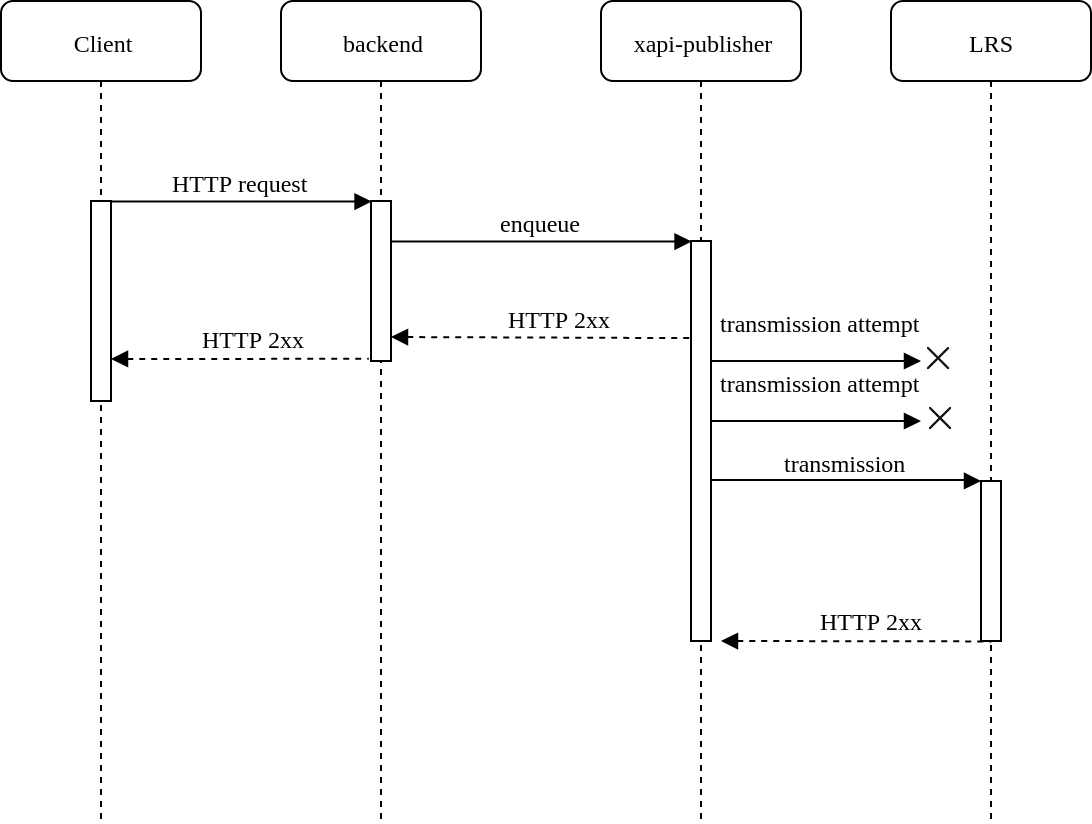
\includegraphics[width=.8\textwidth]{asynchronous-xapi}
            \caption{Asynchronous (non-blocking) transmission of xAPI statements}
            \label{fig:asynchronous-xapi}
        \end{figure}

        Sending of xAPI statements is separated from the API, as sending and
        possible re-transmissions should not block the API from responding
        to requests. This was discovered during testing, when a misconfigured xAPI
        recipient was used. HTTP timeouts are usually in the order of seconds and 
        unsuccessful connection attempts are retried. This resulted in
        the site becoming unresponsive when submitting the survey, as the submission
        of a survey would cause a large number of xAPI statements to be sent.
        Figures \ref{fig:synchronous-xapi} and \ref{fig:asynchronous-xapi} illustrate
        this issue.

\subsection{LTI Middleware}
    As mentioned before, recognition of data subjects uses the same token-based
    mechanism that is also used for recognizing data-client sessions.
    Since session management is performed by the backend service,
    but the frontend bundle is served by the frontend service, performing
    an LTI launch involves both services. The frontend provides an HTTP
    endpoint for requesting the LTI launch. The supplied information
    is then forwarded to the backend service, which validates
    the supplied combination of consumer key and requested questionnaire.
    If the LTI launch is valid, the backend service starts a new session
    for the data subject. A session token is then returned to the frontend
    service. The frontend service embeds the session token as a global
    variable into the JavaScript bundle which is the user interface and
    serves the parameterized bundle to the client.
    The user interface's bootstrapping process may then check for
    the presence of the session token and switch to it's embedded version.
    The embedded version of the user interface uses a different endpoint
    for submitting responses than the standalone version, as no information
    about the data subject has to be present in the response.
    A sequence diagram for the LTI launch is provided in Figure \ref{fig:lti-launch}.

    \begin{figure}
        \centering
        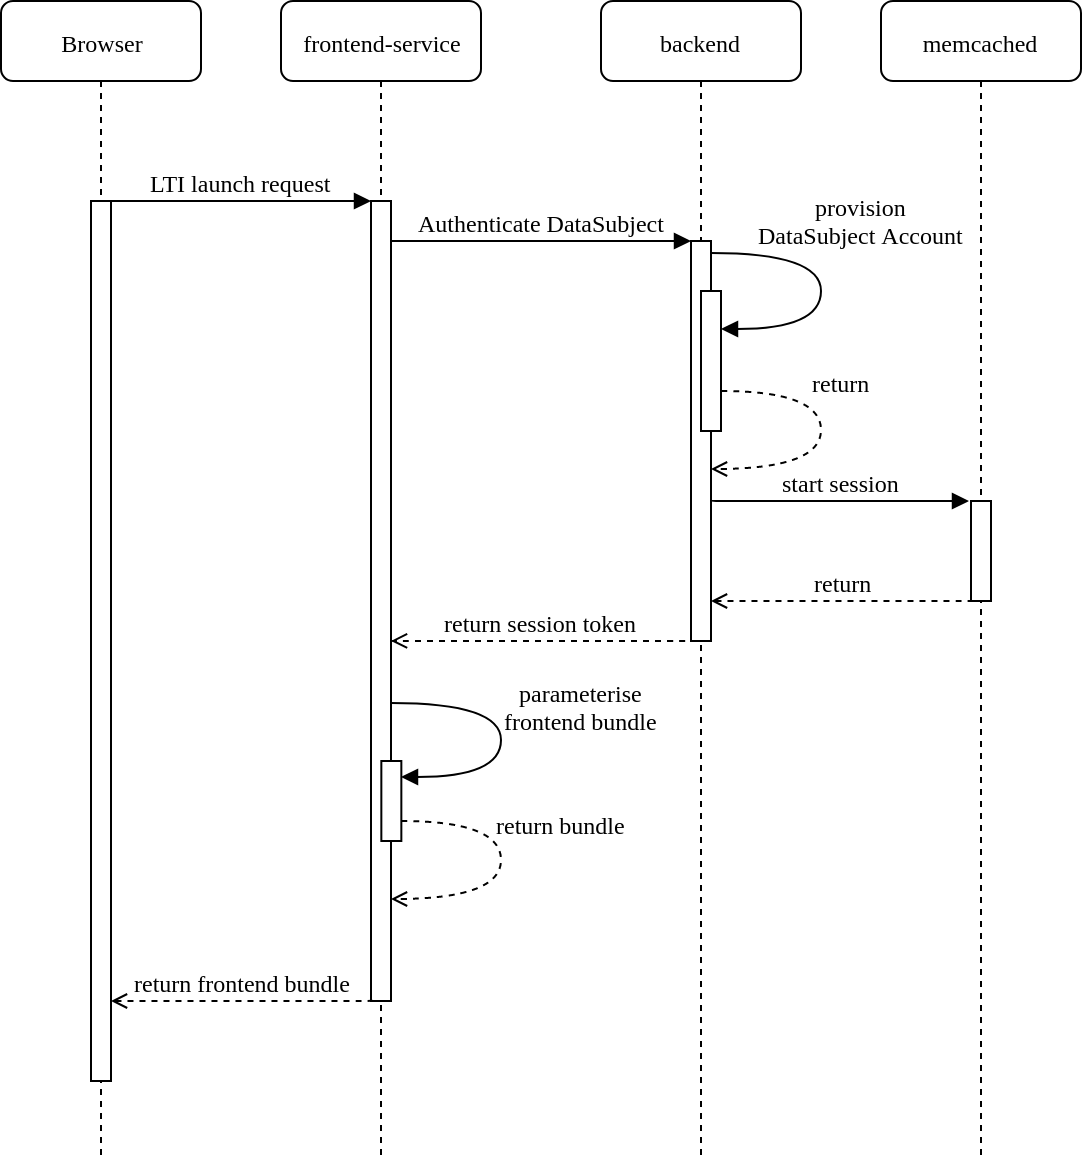
\includegraphics[width=\textwidth]{lti-launch}
        \caption{Sequence diagram depicting the LTI launch}
        \label{fig:lti-launch}
    \end{figure}
    

    \section{Analysis}
    \subsection{Known Issues \& Caveats}
        Joined table inheritance is inferior to single table inheritance
        for this application, even if it looks ugly. Why: performance,
        no foreign key constraints that mess with you

        The template feature is too sophisticated, import and export would have sufficed
        this took time away

        No tests exist for the backend, major burden on maintainability

         the email adress of the data client who conducts the survey
    is added as a prefix to all xAPI activity IDs before sending.
    -> Drawback: not normalized, potential fix: use Instructor <-

    \section{Outlook}
	\subsection{Beta-Testing and Productive Use}
		The survey tool will be used by participants of the Educational Technologies
		Seminar held by Prof. H. Drachsler in the 2018/19 winter semester for the first time.
		In the seminar, students may choose to participate in a test-run
		of the TLA infrastructure. In this test-run, data is gathered
		from different sources, including the survey tool, to test
		the capabilities of the TLA infrastructure and to discover
		potential issues with the system. Participants will
		take a survey accessing motivation and self-regulation
		with regards to their learning behavior. This data will
		then be combined with activity data collected from Moodle,
		regularly self-reported data on goal setting and time management
		and physical attendance times.

	\subsection{Future Features}
		There are many additional features which could be added to
		the existing codebase, once the known issues have been resolved.
		This section describes some of these features and gives a
		brief outline as to how they could be integrated.

		\subsubsection{Configurable Authentication Mechanisms for xAPI Consumers}
			Some xAPI consumers only accept xAPI statements from known
			sources and thus require authentication before statements
			can be transmitted. The xapi-publisher service already supports
			this and bundles statements by destination and authentication mechanism, 
			so that sessions may be re-used. This is not
			described in this thesis, as this was added as part of a hotfix
			in the last days of this thesis. The user interface
			and backend service do not yet support configuration
			by the user for this feature. In the future, the tool
			could provide a set of common authentication mechanisms
			for the data client to choose from. Depending on the
			chosen mechanism, different configuration forms
			would then be displayed in the user interface to supply
			credentials for the mechanism. 

		\subsubsection{Additional Response Types}
			In addition to questions which can be answered on a numerical
			scale, other kinds of response types could be added to the survey
			tool. This is particularly interesting for use cases outside
			psychometry, say, when performing course evaluations.
			Examples for additional response types are free text,
			boolean (yes or no), date \& time and date- \& time-ranges.
			Integrating these kinds of questions would mainly involve
			subclassing the \inline{Question} class and designing
			new user interface components. The overall survey logic
			should still work with these new types. xAPI also already
			supports these kinds of answer values.

		\subsubsection{Additional Formatting Options for Data Clients}
			At the moment, questions present a question text, as
			well as labels for the upper and lower bounds of the response
			range to the data subject. The question text does not
			support formatting. This format is not suited to
			longer paragraphs of text, say, when context has
			to be provided for the question. In the future, questions
			could support formatting using a markup language
			like markdown or textile. The benefit of using such a markup
			language is that no changes have to be made to the way
			question texts are stored, as the markup
			can be stored as plain text. In addition, good library support
			exists for converting these markup languages to HTML
			in a safe manner. In the user interface, the markup
			could either be entered by hand, if the markup language
			is not too complicated, or an already existing
			JavaScript markdown editor like SimpleMDE could be integrated.
			Depending on the markup, this would also allow for images
			and videos to be embedded into the survey, which
			could greatly expand the set of surveys that can
			be realized with the survey tool.

		\subsubsection{A/B Questionnaires}
			Some surveys study the effect of survey taking itself
			on it's subjects. For this reason, different versions
			of the same questionnaire might be presented to
			data subjects. One such example would be a survey,
			where one version uses an even number of response
			values and the other uses an odd number. Currently,
			the entire questionnaire would have to be duplicated in
			order to achieve this. To solve this, a special
			copy of a questionnaire could be created, which is
			also optionally modifiable. Non-modified parts
			of the questionnaire would then merely reflect the
			state of the original questionnaire, whereas modified
			parts would override the original questionnaire's content.
			Participants could then be randomly assigned one of these
			questionnaires when accessing the survey.

		\subsubsection{Version Control for Templates}
			Instead of immediately propagating changes to templates
			to all copies of it, data clients owning a copy
			could be notified of the change and then choose to
			move to the new version or keep using the old one.
			This feature would involve keeping track of
			content revisions for every survey item.
			Instead of overwriting content when making changes
			to a survey item, the changes would instead be
			applied to a copy of the item, the new revision.
			Copies of templates would then also contain information
			about the revision they are shadowing. 
			Up- or downgrading a survey item to another revision
			would then only involve changing the copy's
			\inline{reference_to} relationship to point to the newer
			or older revision.
    \section{Appendix}

    \subsection{Additional Contents}
	\subsubsection{Source Code}
	    The source code for this project is maintained at GitHub and can be found at
	    \url{https://github.com/yeldiRium/st3k101}.
	    The version submitted as part of this thesis is version \inline{3.1.1-beta}, 
	    which can be accessed at \url{http://bit.ly/xapi-probe-311}. There, the
	    source code is available as a zip-compressed archive. The reader may
	    prove the authenticity of the release by calculating the archive's
	    SHA-1 hash sum. \\
	     
	    \inline{st3k101-3.1.1-beta.tar.gz: 7b2dbd474653978331d3263c7c1f2c7c9ff27f63}
	     
	    \inline{st3k101-3.1.1-beta.zip: bc28878196617db812e081c5d48a9e3f689b2714}\\[1em]

	\subsubsection{Documentation}
	    The project's \inline{README} file is the central point of access for information on deployment,
	    dependencies and development setup.
	    It can be accessed at \url{http://bit.ly/xapi-probe-readme}, and is also included
	    in the zip-compressed archive.

	\subsubsection{API Reference}
	    The API reference for the \inline{backend} service can be accessed
	    at \url{http://bit.ly/xapi-probe-api-v6}. This version exists
	    for reference only and will not be updated.

	\pagebreak
	\subsection{List of xAPI Statements}

\begin{figure}[H]
    \begin{lstlisting}[language=JSON]
{
    "actor": {
        "account": {
            "homePage": "http://lmsng.school.edu",
            "name": "292832126.333"
        },
        "name": "292832126.333",
        "objectType": "Agent"
    },
    "context": {
        "contextActivities": {
            "grouping": [
                {
                    "definition": {
                        "description": {
                            "en-US": "This is a survey hosted at st3k101."
                        },
                        "name": {
                            "agq": "Questionnaire name"
                        },
                        "type": "http://id.tincanapi.com/activitytype/survey"
                    },
                    "id": "<bla@blubl.net>:Questionnaire-n-f7f705a0c1",
                    "objectType": "Activity"
                }
            ],
            "parent": [
                {
                    "definition": {
                        "description": {
                            "en-US": "This is a particular scale of a survey, it usually contains multiple questions."
                        },
                        "name": {
                            "de": "4.2 \u00dcberwachung"
                        },
                        "type": "http://fantasy.land/dimension"
                    },
                    "id": "<bla@blubl.net>:lernstrategien_wild_schiefele--4_2_&#252;berwachung",
                    "objectType": "Activity"
                }
            ]
        },
        "language": "agq",
        "platform": "st3k101 via lmsng.school.edu"
    },
    "id": "fcc317f7-d3ce-4597-ad88-245792ecb9c9",
    "object": {
        "definition": {
            "description": {
                "en-US": "This is a question that is part of a survey at st3k101."
    \end{lstlisting}
    \caption{Anatomy of an xAPI statement}
    \label{fig:anatomy-xapi-statement}
\end{figure}

\begin{figure}
    \begin{lstlisting}
            },
            "name": {
                "de": "Ich bearbeite zus\u00e4tzliche Aufgaben, um festzustellen, ob ich den Stoff wirklich verstanden habe."
            },
            "type": "http://adlnet.gov/expapi/activities/question"
        },
        "id": "<bla@blubl.net>:lernstrategien_wild_schiefele--4_2_&#252;berwachung--7",
        "objectType": "Activity"
    },
    "result": [
        {
            "score": {
                "max": 5,
                "min": 1,
                "raw": 2,
                "scaled": 1
            }
        }
    ],
    "timestamp": "2018-10-12T09:41:15.151759",
    "verb": {
        "display": {
            "en-US": "Indicates the DataSubject answered something."
        },
        "id": "http://adlnet.gov/expapi/verbs/answered"
    }
}                 
    \end{lstlisting}
\end{figure}
    
    \pagebreak
    \subsection{Abbreviations}
    \begin{description}
        \item[API] Application programming interface; a software interface for
        interoperability between applications.
        \item[CSV] Comma separated values; a plain-text data exchange format for homogenous
        data.
        \item[ORM] Object-relational-mapper; a software library for persisting objects
        in object-oriented languages in a relational database.
        \item[ODM] Object-document-mapper; a software library for persisting objects
        in object-oriented languages in a document based database.
        \item[xAPI] Experience API, formerly TinCan API; an API specification for
        exchanging data about learning activities.
        \item[REST] Representational state transfer; a paradigm for API design.
        \item[JSON] Javascript object notation; a plain-text data exchange format.
        \item[ACID] Atomicity, consistency, isolation, durability; a set of properties
        for database transaction, aiming to guarantee data validity in the event of failure.
        \item[SQL] Structured query language; a language for interfacing with database systems.
        \item[TLA] Trusted learning analytics; a big data storage and analysis infrastructure
        developed at Prof. H. Drachsler's work group.
        \item[LRS] Learning record store; a big data store for xAPI statements.
        \item[LTI] Learning technologies interoperability; a protocol for integrating third-party
        services with an LMS.
        \item[LMS] Learning management system; a content management system specifically
        designed for learning environments.
        \item[CAS] Central authentication service; the user authentication service provided
        by Goethe University's HRZ.
        \item[HRZ] Hochschulrechenzentrum; Goethe University's data center and IT service provider.
    \end{description}

    \pagebreak
    
    \listoffigures
    \listoftables
    \bibliographystyle{alphadin}
    \bibliography{ba.bib}
    
    \end{document}
